%!TEX root = ../dissertation.tex

\chapter{Results}
\label{chp:results}

In this Section I show the results of my thesis work, going from the initial dataset processing, through the model tuning, training and validation and finishing with the results of my proposed explainability framework applied to the given datasets.

\section{GNN experiments}
		In the first part of this section I present the results related to the heterogeneous predictive model implemented. I begin by showing the results of the model's hyperparameter sweep. Then, I provide a comparison of its learning curve against the homogeneous implementation to better understand the effects of using a heterogeneous model instead of a homogeneous one. Finally, I provide a summary of the results of the model against all other baselines for a full comparison.

        \subsection{Hyperparameter sweep}
            \begin{figure}[t!]
                \centering
                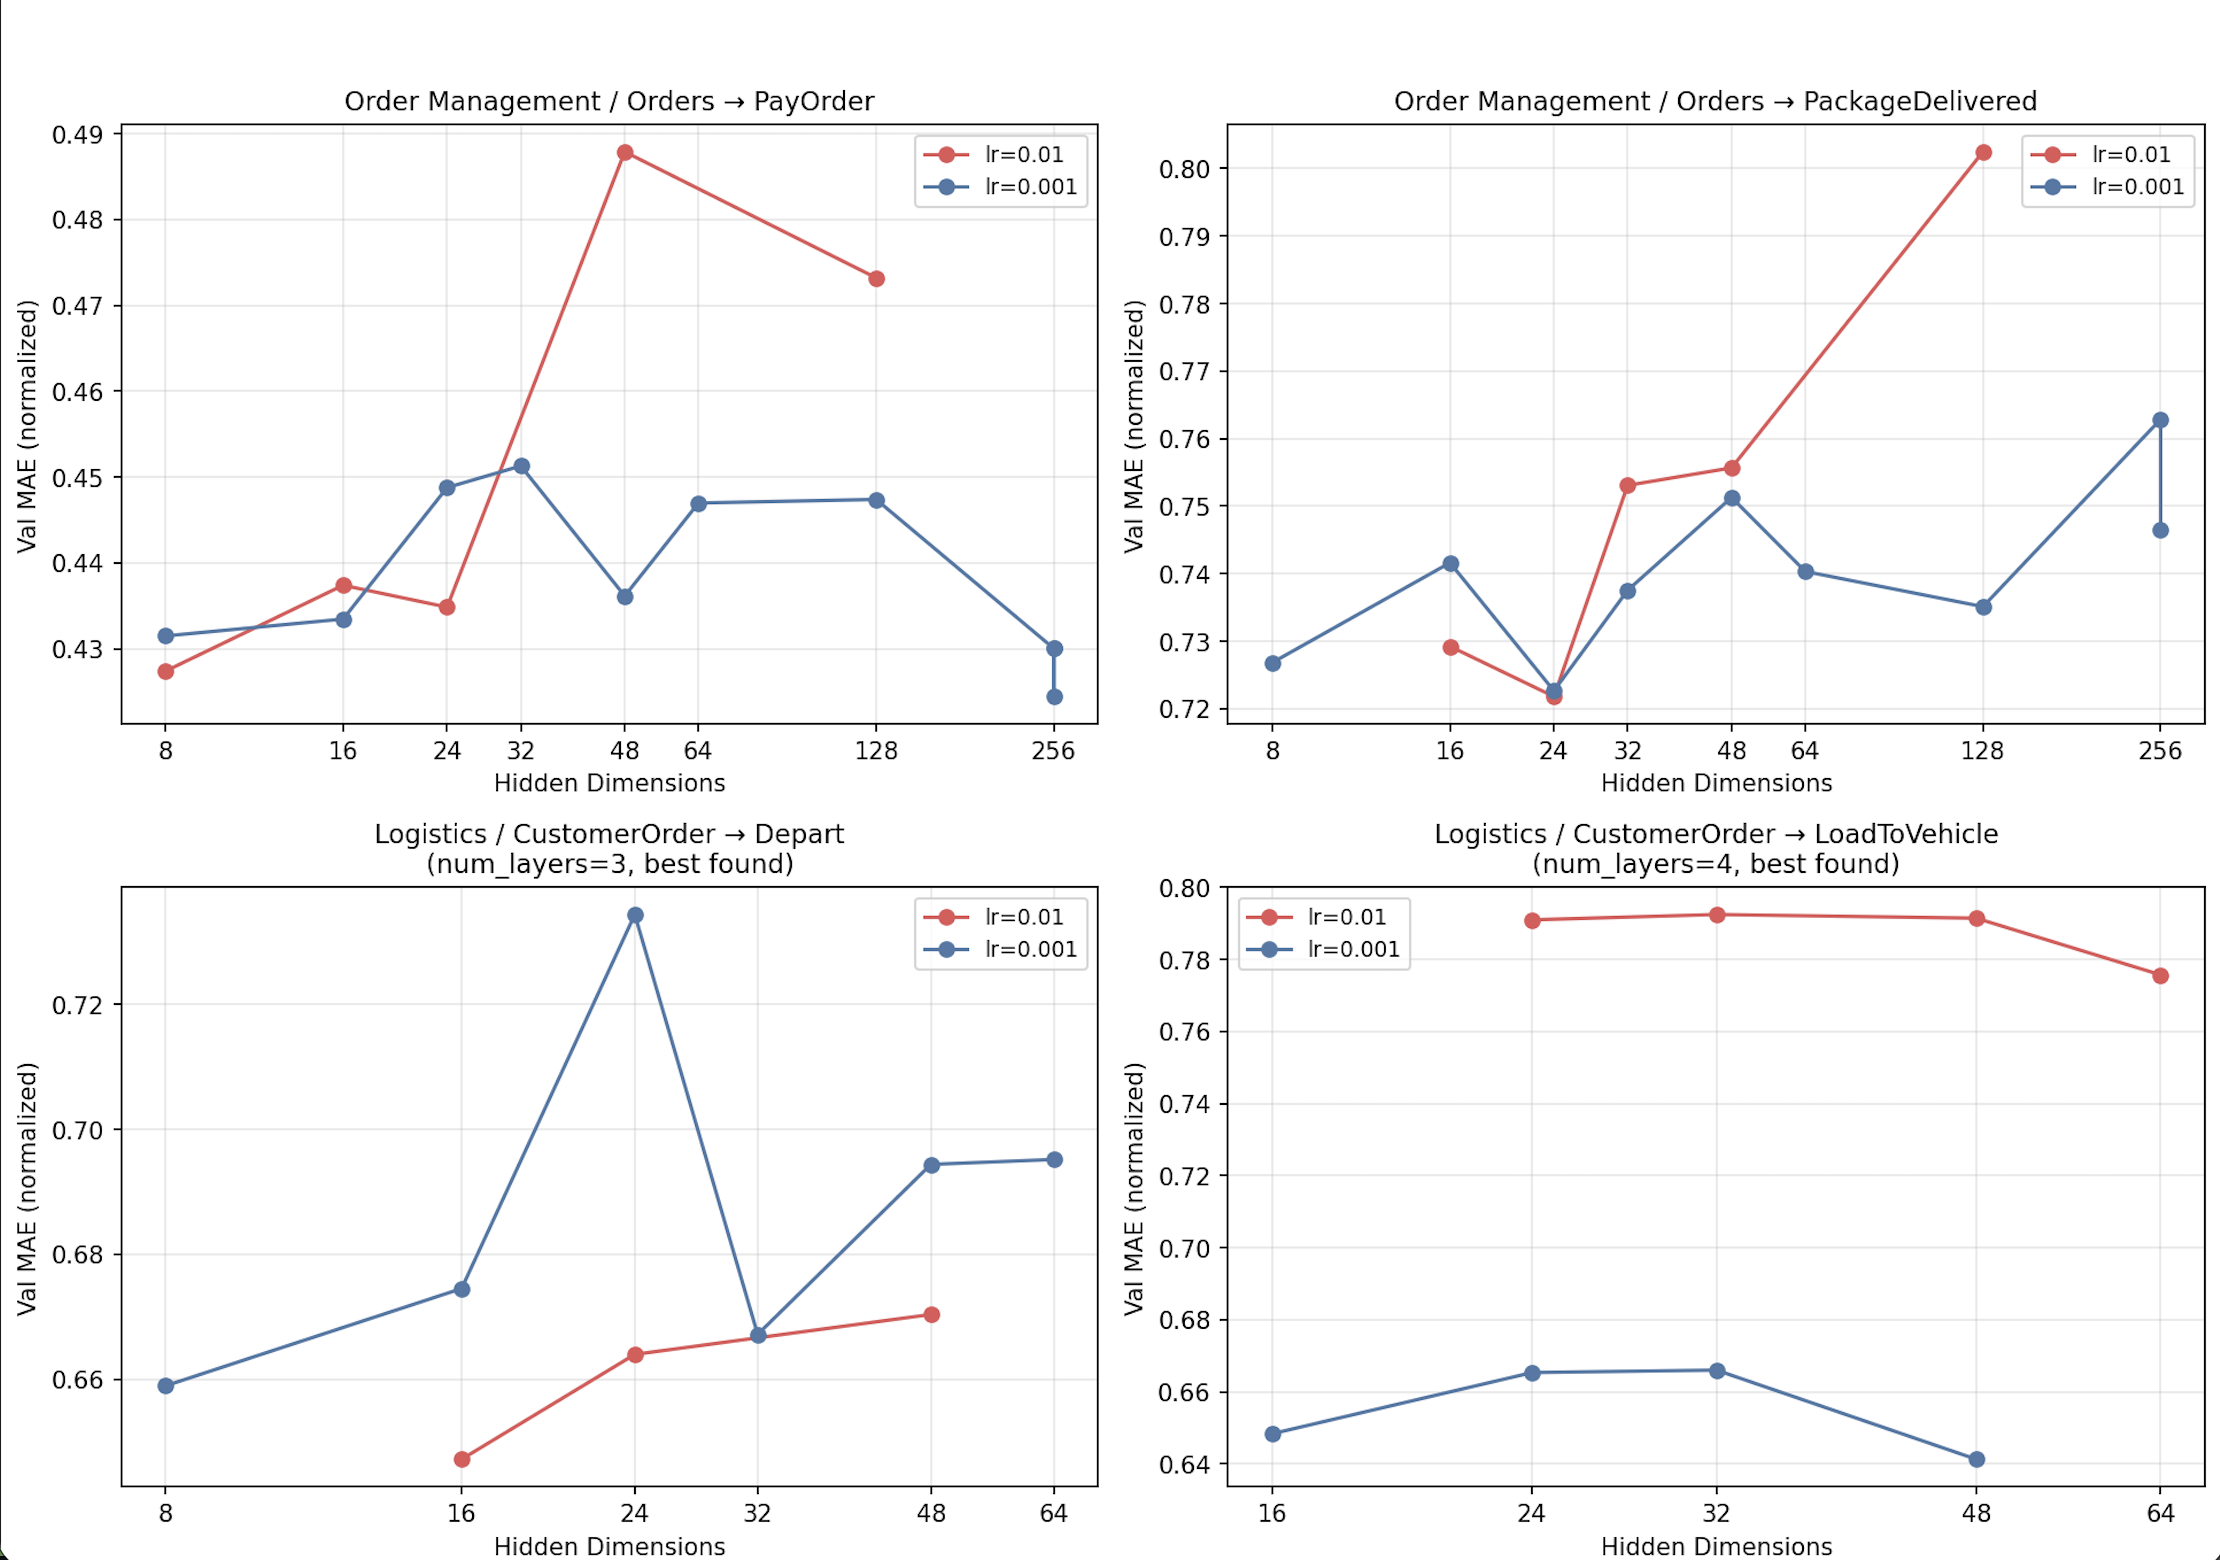
\includegraphics[width=1\textwidth]{figures/hyperparameter_sweep_summary.png}
                \caption{Normalized Val MAE scores for the HTG model per hyperparameter setting. Note: scales (y-axis) are not aligned, as I intended to compare hyperparameter settings within each KPI.}
                \label{fig:hyper_sweep}
            \end{figure}
            
            Fig. \ref{fig:hyper_sweep} shows the effect of tuning the learning rate and the number of hidden dimensions for the HGT regression models used. The graphs show the sweep for each of the four KPIs chosen, with "Orders -> PayOrder" representing the "Elapsed time from Orders to PayOrder" KPI (This nomenclature was used to avoid overloading the graphs with text) and the other three KPIs following the same style.
            
            Beginning with the two graphs shown at the top, referring to the Order Management KPIs, a first observation shows a great difference in volatility between the models' validation error when trained on the 0.01 learning rate versus the lower 0.001 value. The first continues increasing as more hidden dimensions are added, whereas the second is much more stable. It's important to note that the validation error is also higher for the "Elapsed time from Orders to PackageDelivered" KPI as opposed to the values shown for "Elapsed time from Orders to PayOrder" KPI. This could be a result of the difference in process execution length for each given KPI. A notable difference between each KPI model is the chosen hidden dimension value for their respective models, with the "Elapsed time from Orders to PackageDelivered" KPI showing better results with 24 hidden dimensions whereas the "Elapsed time from Orders to PayOrder" KPI showed the best results with the maximum 256 hidden dimensions.

            In order to perform the same sweep on the Logistics database it was first necessary to identify the proper number of layers needed to avoid the problem outlined in Section \ref{sec:dataset_logistics}.
            
            \begin{figure}[t!]
                \centering
                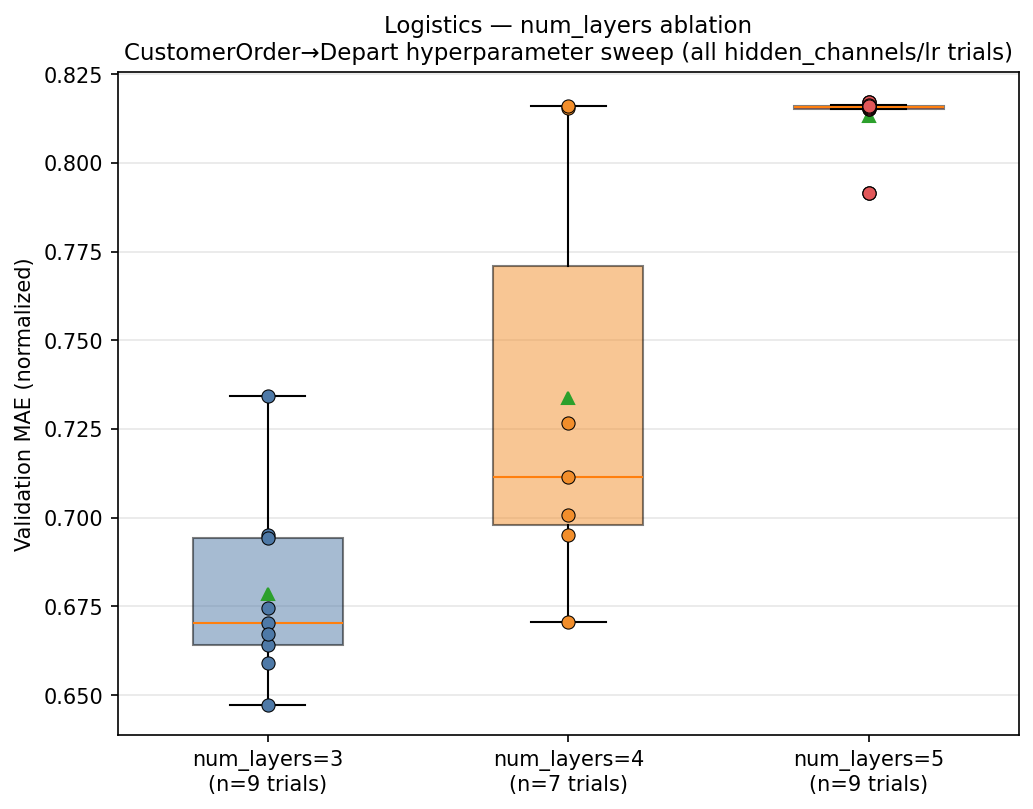
\includegraphics[width=1\textwidth]{figures/depart_ablation.png}
                \caption{Normalized Val MAE scores for the HGT model on the Logistics dataset for KPI "Elapsed time from CustomerOrder to Depart" per different number of layers}
                \label{fig:log_ablation_1}
            \end{figure}

            \begin{figure}[t!]
                \centering
                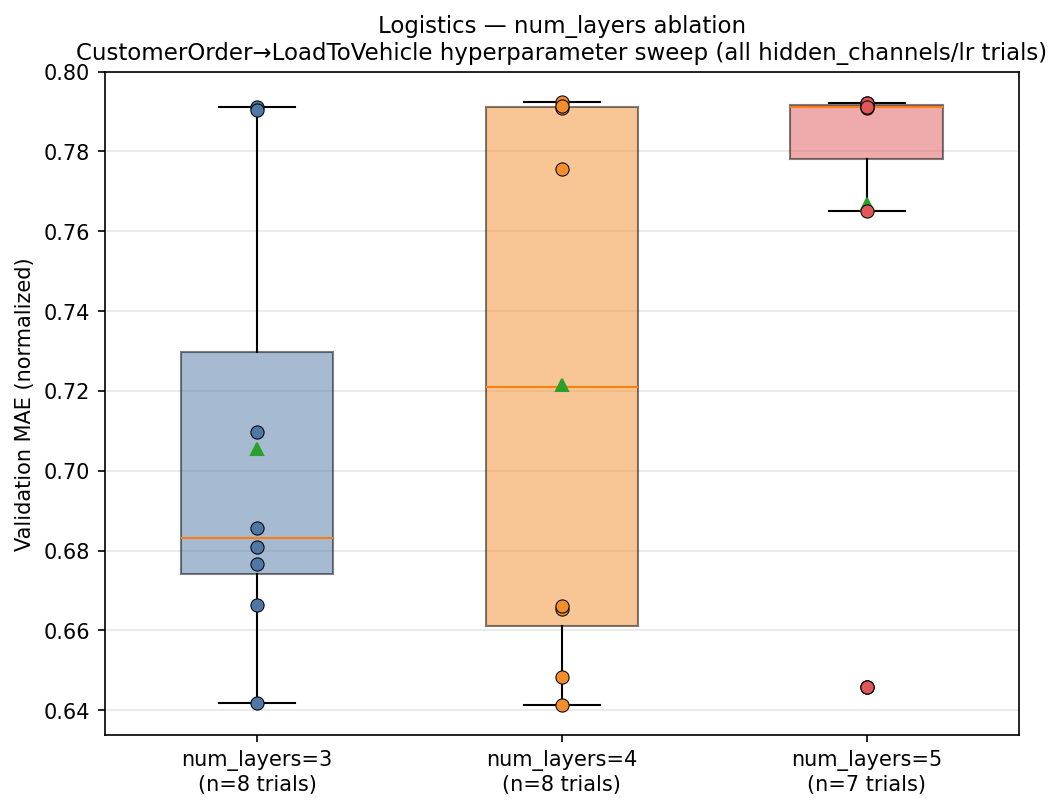
\includegraphics[width=1\textwidth]{figures/loadtovehcile_ablation.png}
                \caption{Normalized Val MAE scores for the HGT model on the Logistics dataset for KPI "Elapsed time from CustomerOrder to LoadToVehicle" per different number of layers}
                \label{fig:log_ablation_2}
            \end{figure}
            
            Fig. \ref{fig:log_ablation_1} and Fig. \ref{fig:log_ablation_2} show the result of the initial sweeps performed over all possible hidden channels and learning rates for each KPI in the Logistics dataset. In Fig. \ref{fig:log_ablation_1} it is evident that 3 layers offers the lowest overall validation error and the resulting sweep selected this value as the best hyperparameter. On the other hand Fig. \ref{fig:log_ablation_2} shows a different case, while the ablation analysis shows the number of layers at 3 having the best results, with its median at 0.683 versus the 0.721 of 4 layers, the complete sweep eventually selected 4 layers as the best option.

            The second set of graphs in Fig. \ref{fig:hyper_sweep} show the result of the sweep performed on the Logistics KPIs once the number of layers were set at the appropriate value of 3 and 4 respectively. It is important to note the different y-axis scales used by each graph as they are only intended for comparing setting within the model. Looking at the graph its evident that, in contrast to Order Management's results, the Logistics-trained models don't have a generally agreed upon set of hyperparameters characteristics. The "Elapsed time from CustomerOrder to Depart" KPI shows considerably better results when using a higher learning rate and a smaller number of hidden dimensions than either of the Order Management models. However, the sweep for "Elapsed time from CustomerOrder to LoadToVehicle" KPI shows a much flatter curve where the best values are provided by the lower learning rate and a hidden dimension value of 48.

        \subsection{Model comparison versus homogeneous GNN}
        \begin{figure}[t!]
            \centering
            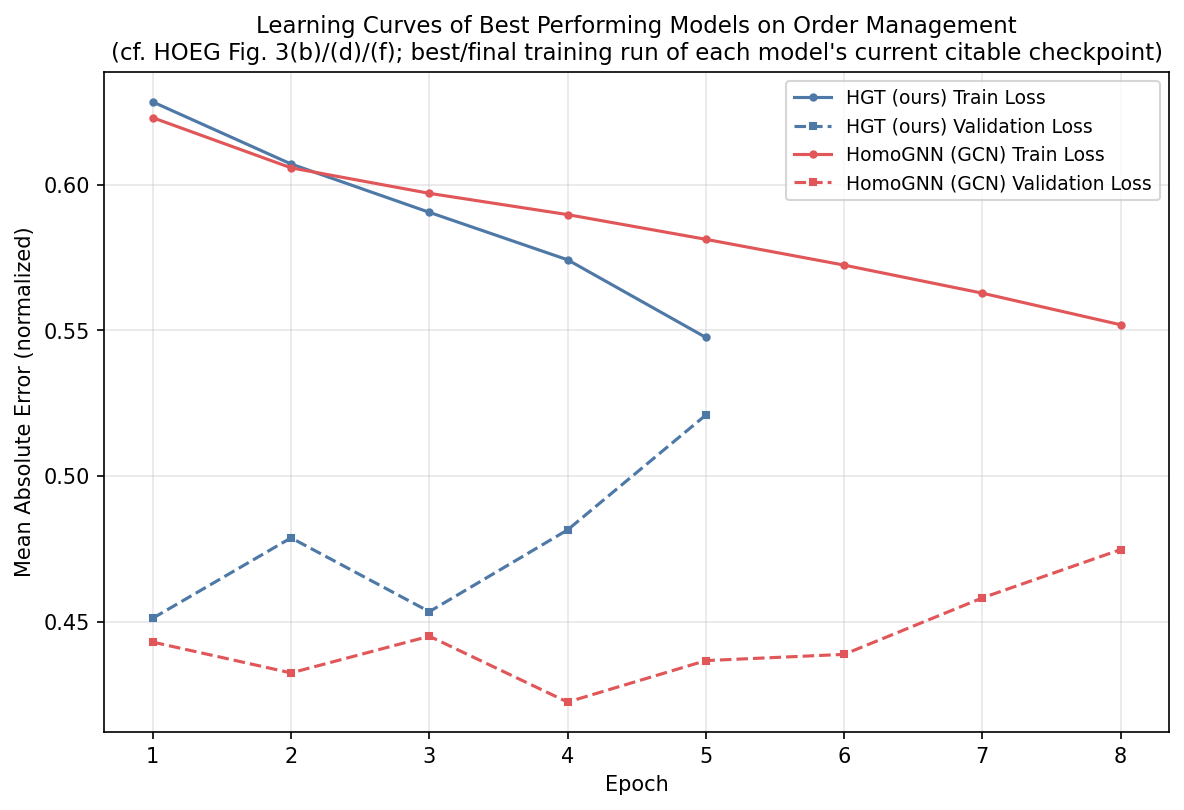
\includegraphics[width=1\textwidth]{figures/training_curves_order_management.png}
            \caption{Training and validation loss learning curves of the trained HGT model and the homogeneous GNN on the best performing model of the Order Management dataset.}
            \label{fig:learning_curves_om}
        \end{figure}
        
        Fig. \ref{fig:learning_curves_om} shows the learning curves for the best performing regression model on the Order Management dataset, which is associated with the prediction of the "Elapsed time from Orders to PayOrder" KPI. As can be seen in the curves, even after performing a hyperparameter sweep the model cannot be improved below a 0.45 MAE. Notably, training loss stays above validation loss for the entire run rather than the reverse, which at first glance suggests overfitting; however, re-evaluating the fully-trained checkpoint directly on each split (rather than reading the pattern off the epoch-by-epoch curve) shows train MAE (388.0 hours) is genuinely higher than validation MAE (353.2 hours), with test MAE the worst of the three (421.2 hours). 
        I then compared each split's target distribution directly, independent of any trained model, to validate whether this behavior was tied to the data source itself. I found the validation window's remaining-time values to be intrinsically less variable than the training window's (standard deviation of 135.8 hours versus 219.6 hours), so even a constant mean-predictor would score better on validation (105.7 hours MAE) than on training (158.1 hours MAE) suggesting temporal drift in the dataset.
        Test's higher error similarly reflects genuine temporal drift toward longer remaining times later in the dataset's timeline, not a generalization failure. Two candidate explanations for the pattern were checked directly and ruled out. The first was the possibility that the gap was caused by the z-normalization statistics being fit only on the training split. However, the denormalized MAE metric already corrects for this uniformly across splits so this explanation was discarded. Secondly, this pattern could be caused by too few training epochs. However, this explanation was also discarded since the gap traces to an intrinsic property of each split's data rather than an undertrained model. Training was still halted once the early-stop trigger activated after validation MAE stopped improving. The homogeneous implementation, which is allowed to train for longer, shows a similar overall pattern, with a decrease in training error not producing a decrease in validation error, instead increasing again after finding its local minimum at epoch 4 until it's also cut off by the early-stop trigger. Its smoother-looking curve does not translate into a clear performance advantage over the heterogeneous model for this KPI. HomoGNN's all-prefix MAE is slightly lower (157.5 hours versus 167.1 hours), but its last-event MAE remains higher than the heterogeneous model's (103.8 hours versus 98.0 hours). A full baseline comparison is presented later in this chapter that provides a complete picture across both metrics.

        

        \begin{figure}[t!]
            \centering
            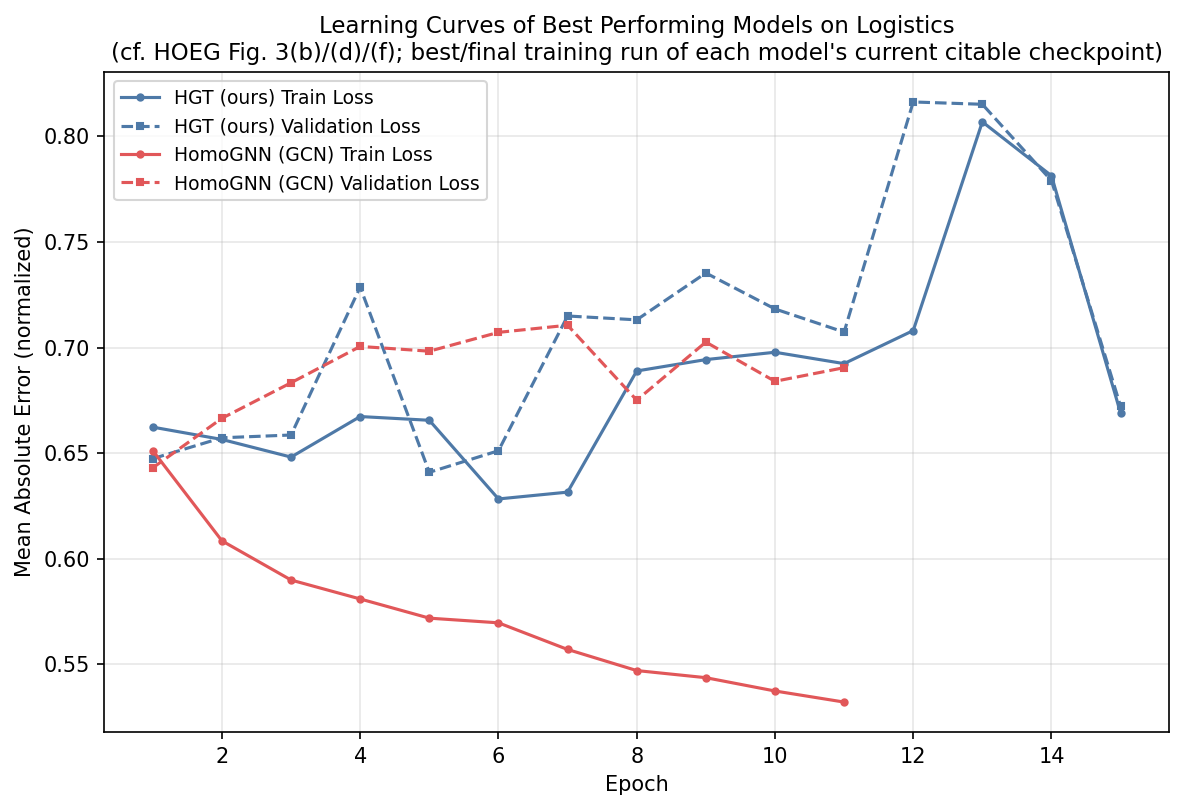
\includegraphics[width=1\textwidth]{figures/training_curves_logistics.png}
            \caption{Training and validation loss learning curves of the trained HGT model and the homogeneous GNN on the best performing model of the Logistics dataset.}
            \label{fig:learning_curves_log}
        \end{figure}

        Fig. \ref{fig:learning_curves_log} shows the learning curves for the best performing regression model on the Logistics dataset, which is associated with the prediction of the "Elapsed time from CustomerOrder to Depart" KPI. Both the homogeneous and heterogeneous models show a genuine overfitting-like divergence toward the end of the plotted run, with validation loss rising as training loss keeps dropping, and neither curve having visibly stabilized by the final epoch shown. 
        This divergence, however, occurs entirely after the epoch that early stopping actually selected. Logistics uses a patience of 10 epochs, so the plotted curve necessarily extends 10 epochs beyond the checkpoint that was saved and is cited elsewhere in this thesis, and it is in those extra, discarded epochs that training loss continues falling while validation loss rises. By reloading the actually-deployed checkpoint and re-evaluating it directly I confirmed that it does not carry this gap. Train, validation and test MAE are all within about 8 hours of each other (432.1h/435.1h/439.9h). Unlike what can be seen in the results for the order management dataset for this dataset the two models track each other closely throughout.

        Overall, neither graph reflects classic overfitting once the pattern behind it is more closely analyzed. Order Management's apparent gap is a property of its temporal validation split rather than a generalization failure, and Logistics' apparent divergence occurs only in training epochs beyond the one actually deployed. What both datasets do share is a training process that plateaus early, with the best available hyperparameters still leaving both model architectures at a relatively high absolute MAE floor for their respective KPIs.

        \subsection{Model comparison against baselines}
        \begin{figure}[t!]
            \centering
            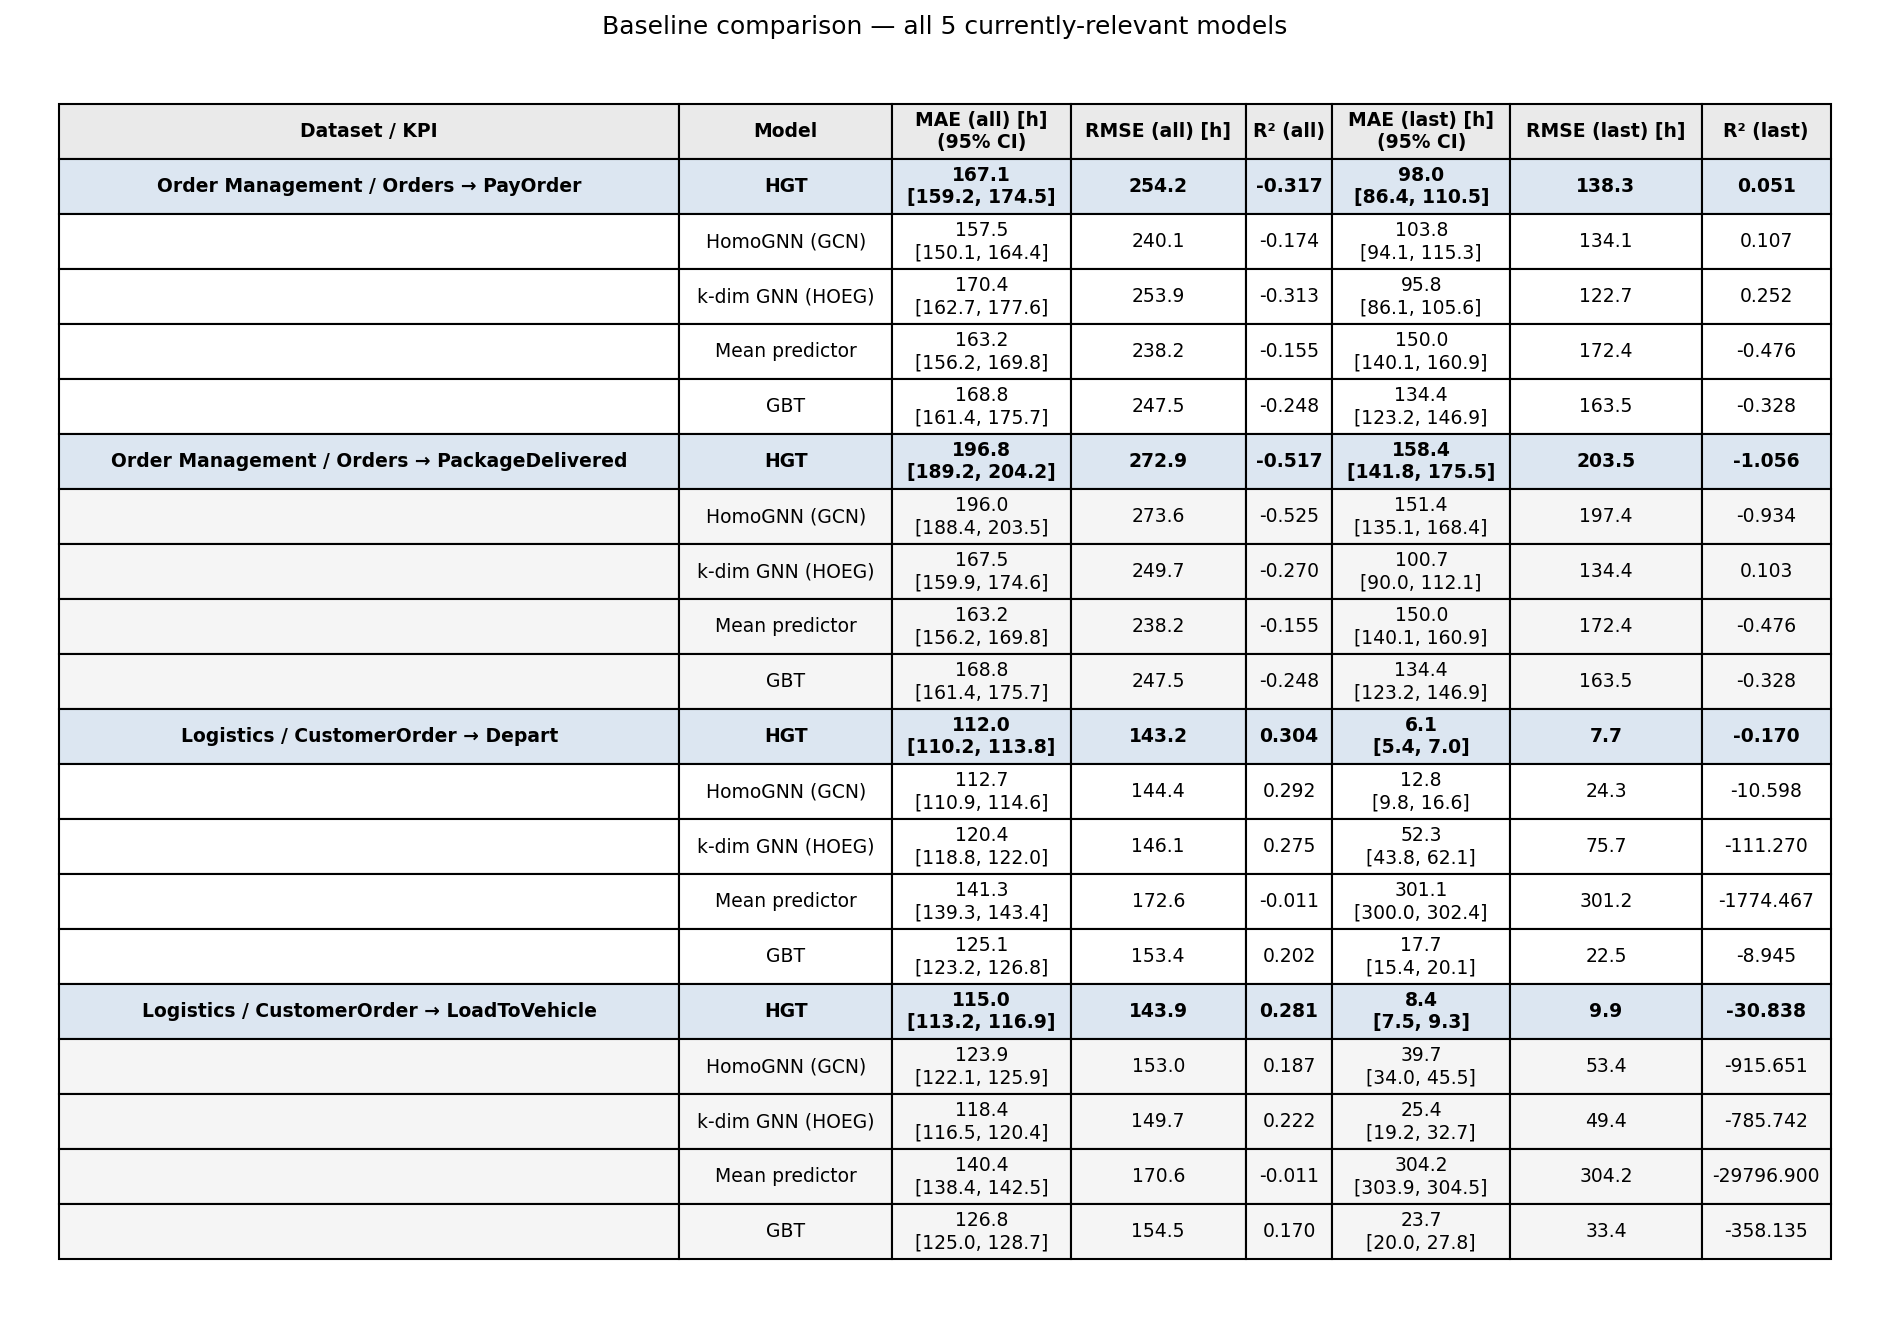
\includegraphics[width=1\textwidth]{figures/combined_baseline_comparison_table.png}
            \caption{Performance of the chosen HGT model and three baseline models. Note: the best-performing hyperparameter configurations are used for HGT}
            \label{fig:baselines}
        \end{figure}
        
        I compared the heterogeneous model against three other implementations: the mean, a Gradient Boosted Trees model and a homogeneous implementation of the dataset. By comparing the performance to these baseline models I wanted to understand how well the heterogeneous implementation stacked up to other options.
        Fig. \ref{fig:baselines} shows the results, with the MAE value denormalized and shown as hours. As I explained in Section \ref{sec:models_baselines} I was interested in checking the quality of the model not only on the entire prefix set but also as the prefix depth increased to evaluate if the increase in information was leading to an increase in predictive quality, Therefore, the graph presents the MAE values for both, the model tested on every prefix in the testing set as well as only those marked as Last-Event prefixes, which contain the maximum amount of information possible about the process execution.

As expected, the median estimator shows the worst overall performance for two of the four KPIs ("Time from CustomerOrder to Depart" and "Time from CustomerOrder to LoadToVehicle"). For the other two, however, it instead outperforms both the heterogeneous model and GBT: its error is slightly below both on "Time from Orders to PayOrder," and it is in fact the single best-performing model of the four on "Time from Orders to PackageDelivered." GBT's own performance is similarly inconsistent across KPIs rather than uniformly ranked: it is the single worst-performing model on PayOrder, the second-best (behind only the median estimator) on PackageDelivered, and mid-pack on the two Logistics KPIs, beating only the median estimator on each of those.
        Comparing the graph-based models it's clear that neither model can be identified as truly better than the other, with their respective accuracy values being very close. Looking at the confidence intervals of each model also shows that both models tend to have overlapping estimate ranges. Therefore, given the spread between models, it cannot be claimed with certainty that the heterogeneous representation is head-and-shoulders above the others — only that it is a reasonable, comfortable prediction.

        This changes if we compare the models only on the last-event prefix, though not as uniformly as it may first appear. For two of the four KPIs ("Time from CustomerOrder to Depart" and "Time from CustomerOrder to LoadToVehicle") the heterogeneous model is significantly more accurate than every baseline (Wilcoxon signed-rank p < 0.001 against each of the three baselines and the k-dim GNN comparison introduced in Section \ref{sec:models_baselines}). For "Time from Orders to PayOrder" it is significantly better than the homogeneous GNN, the mean predictor, and GBT, but statistically indistinguishable from the k-dim GNN baseline (p=0.31). For "Time from Orders to PackageDelivered," the heterogeneous model does not win at all: it is statistically tied with the homogeneous GNN (p=0.48) and significantly less accurate than the mean predictor, GBT, and the k-dim GNN baseline. 
        One further caveat applies on top of this for "Time from CustomerOrder to LoadToVehicle" KPI, which has a strongly negative $R^2$ for every model, most extremely for the mean predictor (R²=-29796). This is a consequence of the last-event target's true scale being tiny, with a mean of 2.3 hours and a standard deviation of only 1.8 hours (an order of magnitude smaller than the other Logistics KPI, which has a mean of 27 hours and a standard deviation of 7 hours). Since $R^2$ is calculated against this tiny variance, even the heterogeneous model's own comparatively modest last-event error produces a negative R² (-30.8)smaller in magnitude than the baselines' because its MAE is itself the lowest of the five, but still negative for the same structural reason. Overall, MAE remains the more informative metric for this KPI. As shown above, the heterogeneous model's last-event MAE is significantly lower than every baseline's here, unlike the mixed picture for PayOrder and PackageDelivered.

        \begin{figure}[t!]
            \centering
            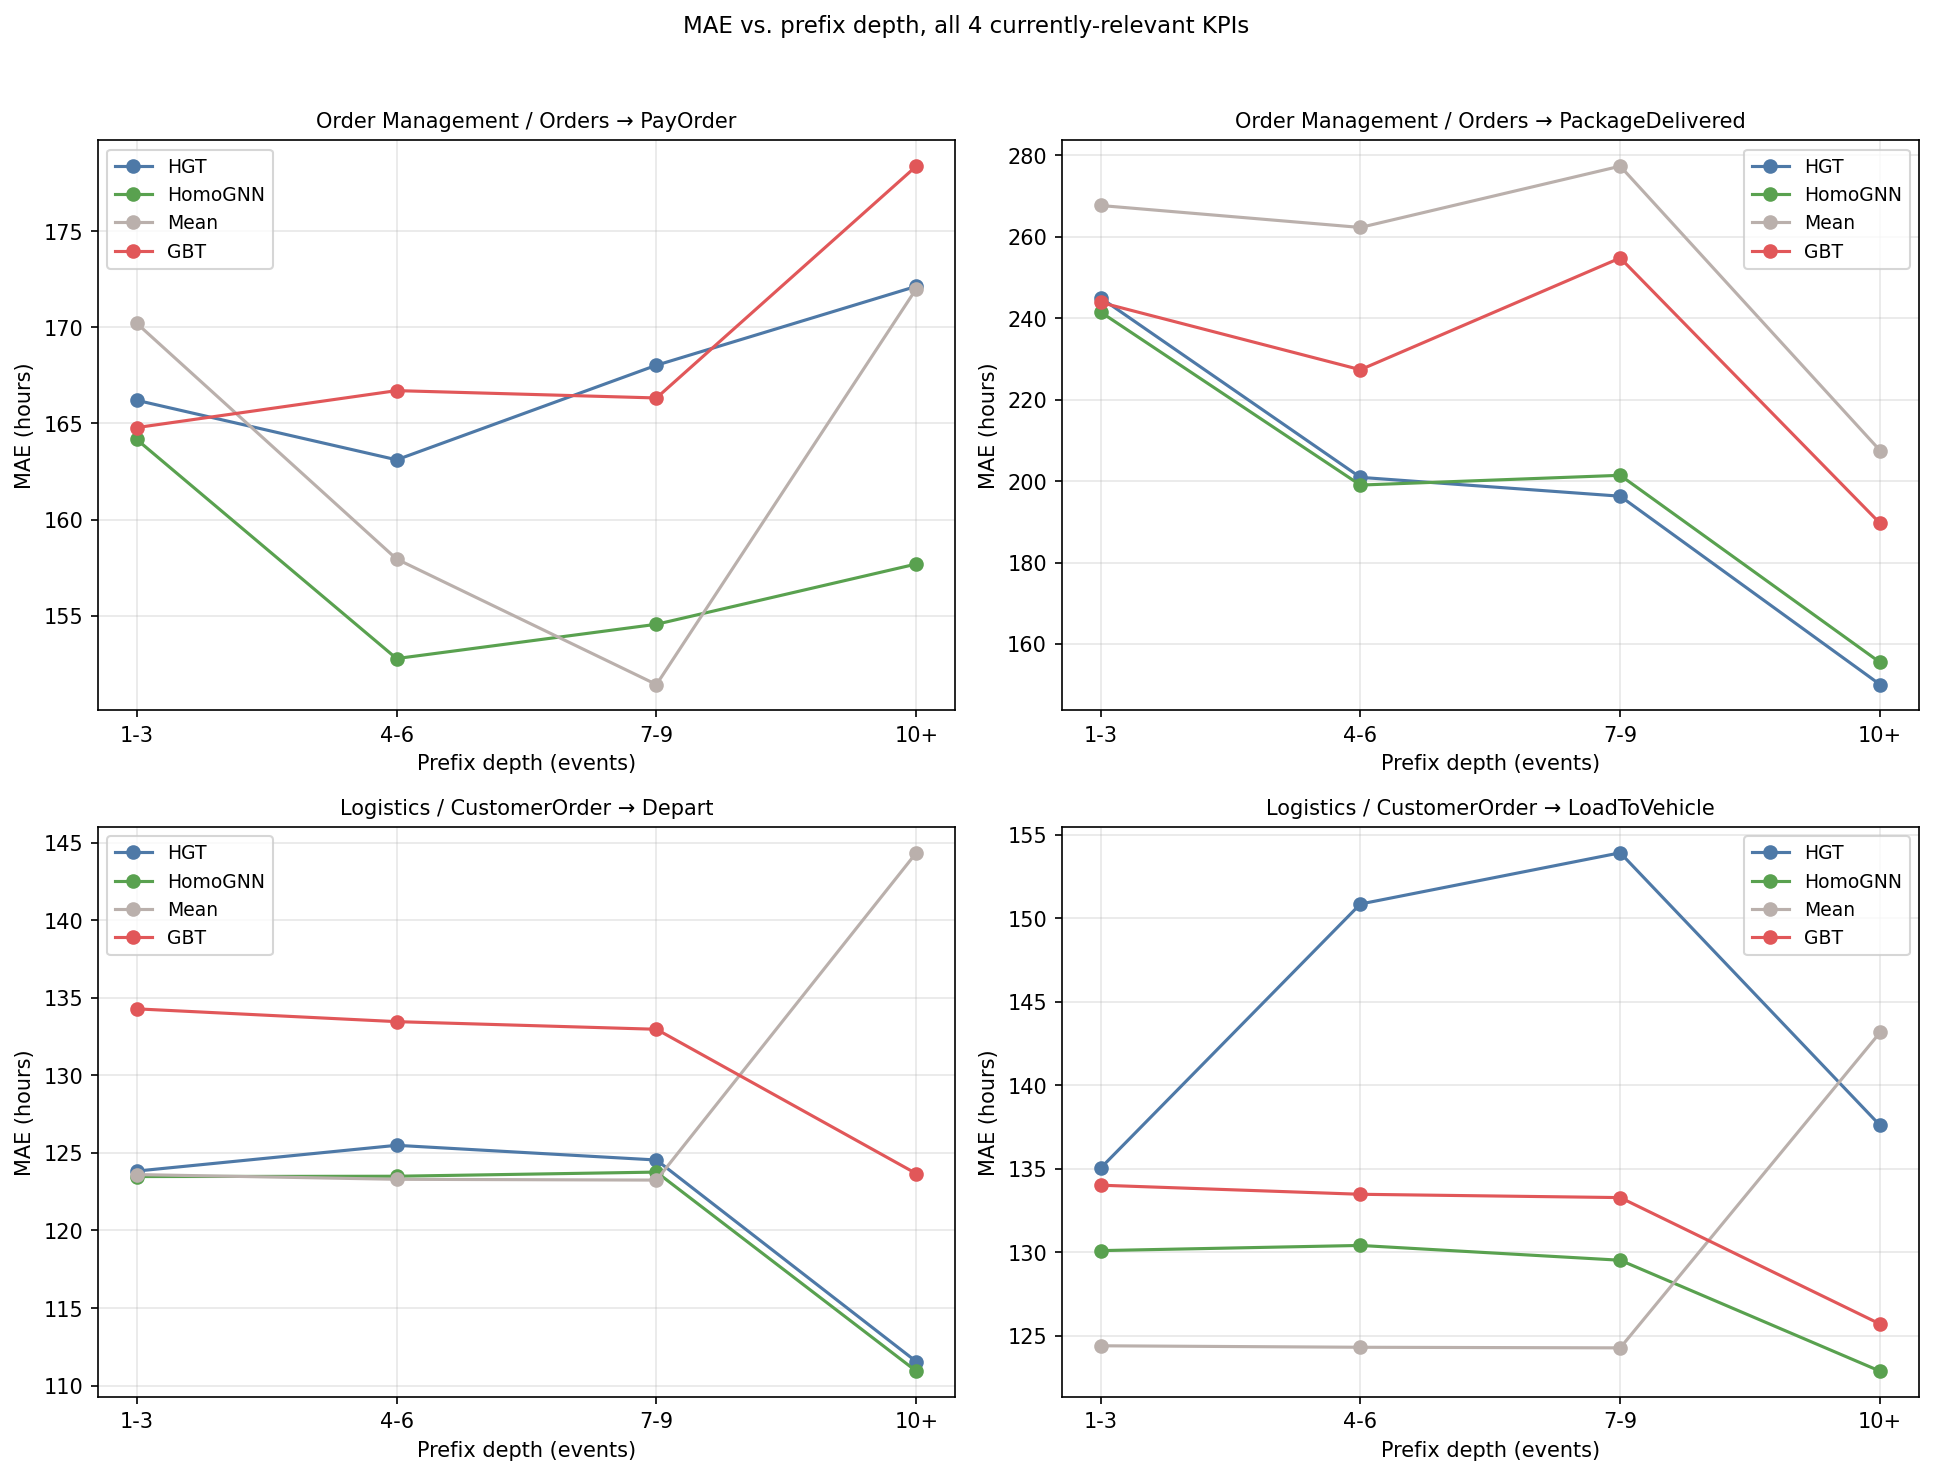
\includegraphics[width=1\textwidth]{figures/mae_by_depth_summary.png}
            \caption{Test MAE for each regression model across prefix depth.}
            \label{fig:depth_summary}
        \end{figure}
        
        Fig. \ref{fig:depth_summary} shows this change in predictive quality over prefix depth. The graphs show that in only two of the four KPIs the model's performance works as expected, with the MAE value decreasing as more information is added to the process execution. The HGT model for the "Time from CustomerOrder to LoadToVehicle" KPI is especially problematic as it's the only model that increases across the prefix depth.
        These graphs also highlight an important result. The HGT model used performs worse for three of the four regression models, with its MAE always higher than the homogeneous model's across multiple prefix depths. 
        This result reverses for two of the four KPIs when comparing the models exclusively on last-event prefixes, as shown in the statistical breakdown above, indicating that aggregate metrics, which are dominated by non-last-event prefixes, and last-event-specific metrics can move independently, sometimes in opposite directions. However, it is worth noting that the aformentioned breakdown also shows this reversal is itself KPI-dependent rather than universal.

    \section{Explainability framework}
        Having described the predictive model's results I now show the results of applying my proposed explainability framework on the created models. I show the output of each of the four distinct components of the framework as well as a short explanation of how the provided explanations can be interpreted by a stakeholder.

        \subsection{Perturbation-based explanation}
            \begin{figure}[t!]
                \centering
                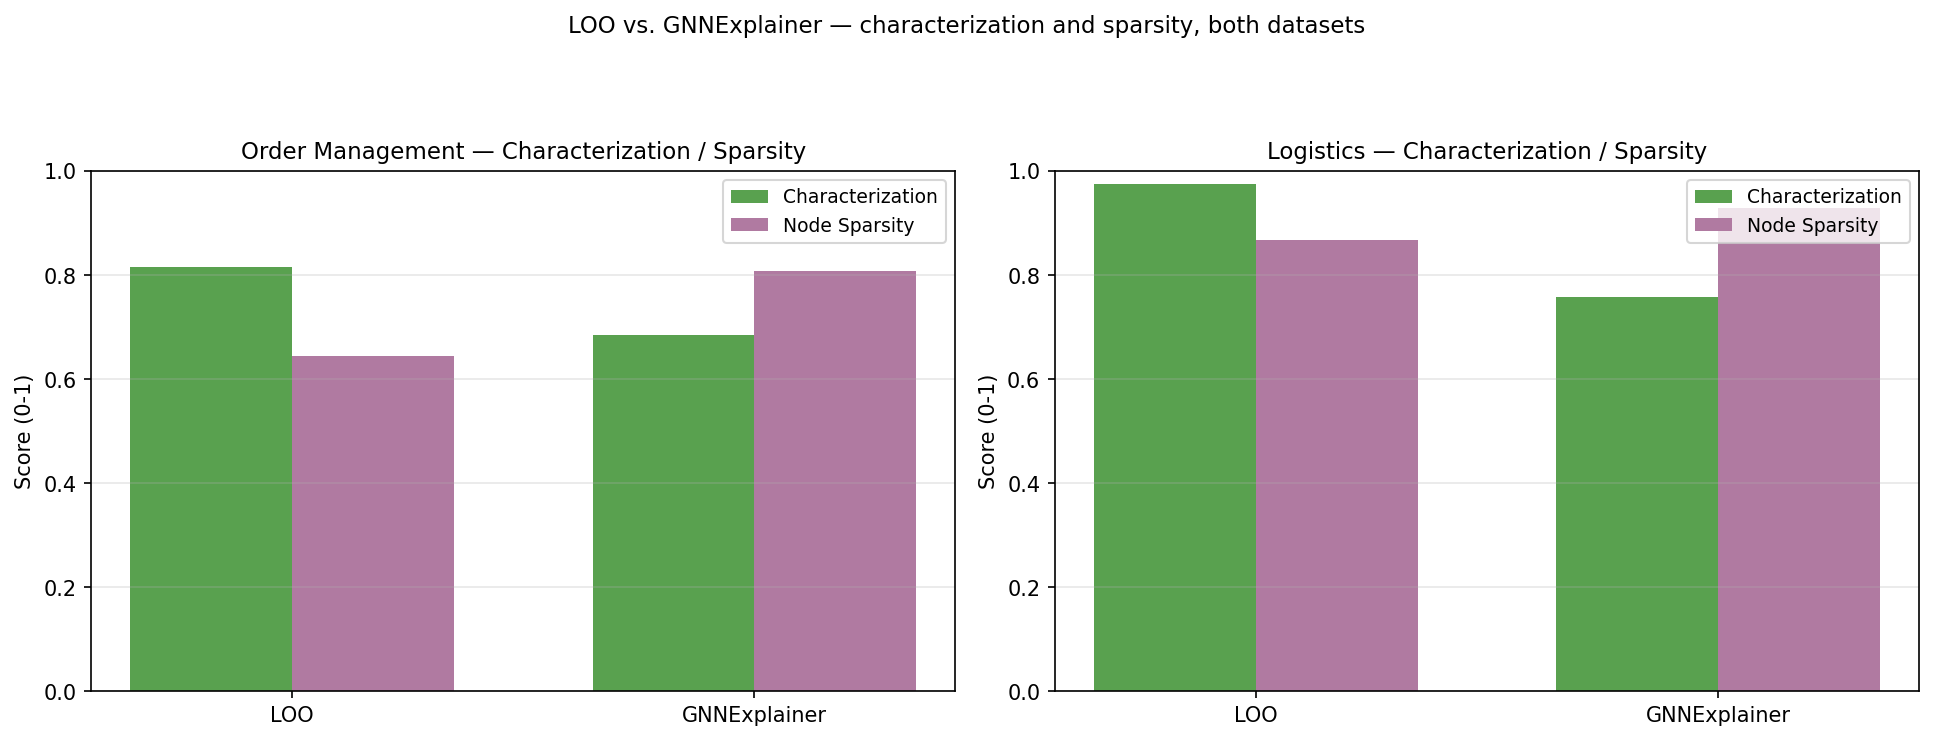
\includegraphics[width=1\textwidth]{figures/fidelity_comparison_summary.png}
                \caption{Fidelity metrics of LOO method against GNNExplainer for KPIs of each dataset}
                \label{fig:loo_comparison}
            \end{figure}
            
			As I explained in Section \ref{sec:dataset_perturb} I performed a series of tests to validate a change in the way this part of the methodology generated its results. Fig. \ref{fig:loo_comparison} shows the results of this evaluation. I compared the two methods on two explanation fidelity metrics: characterization and sparsity. As can be seen LOO outperformed GNNExplainer on both metrics across both datasets (characterization: Order Management LOO 0.815 vs. GNNExplainer 0.685; Logistics LOO 0.975 vs. GNNExplainer 0.757), meaning that features identified through LOO lead to better fidelity metrics compared to those found by the heterogeneous implementation of GNNExplainer. Logistics' characterization score is, in fact, the higher of the two datasets rather than the lower one, indicating that LOO-identified features are highly decisive for the model's prediction in both settings.

            \begin{figure}[t!]
                \centering
                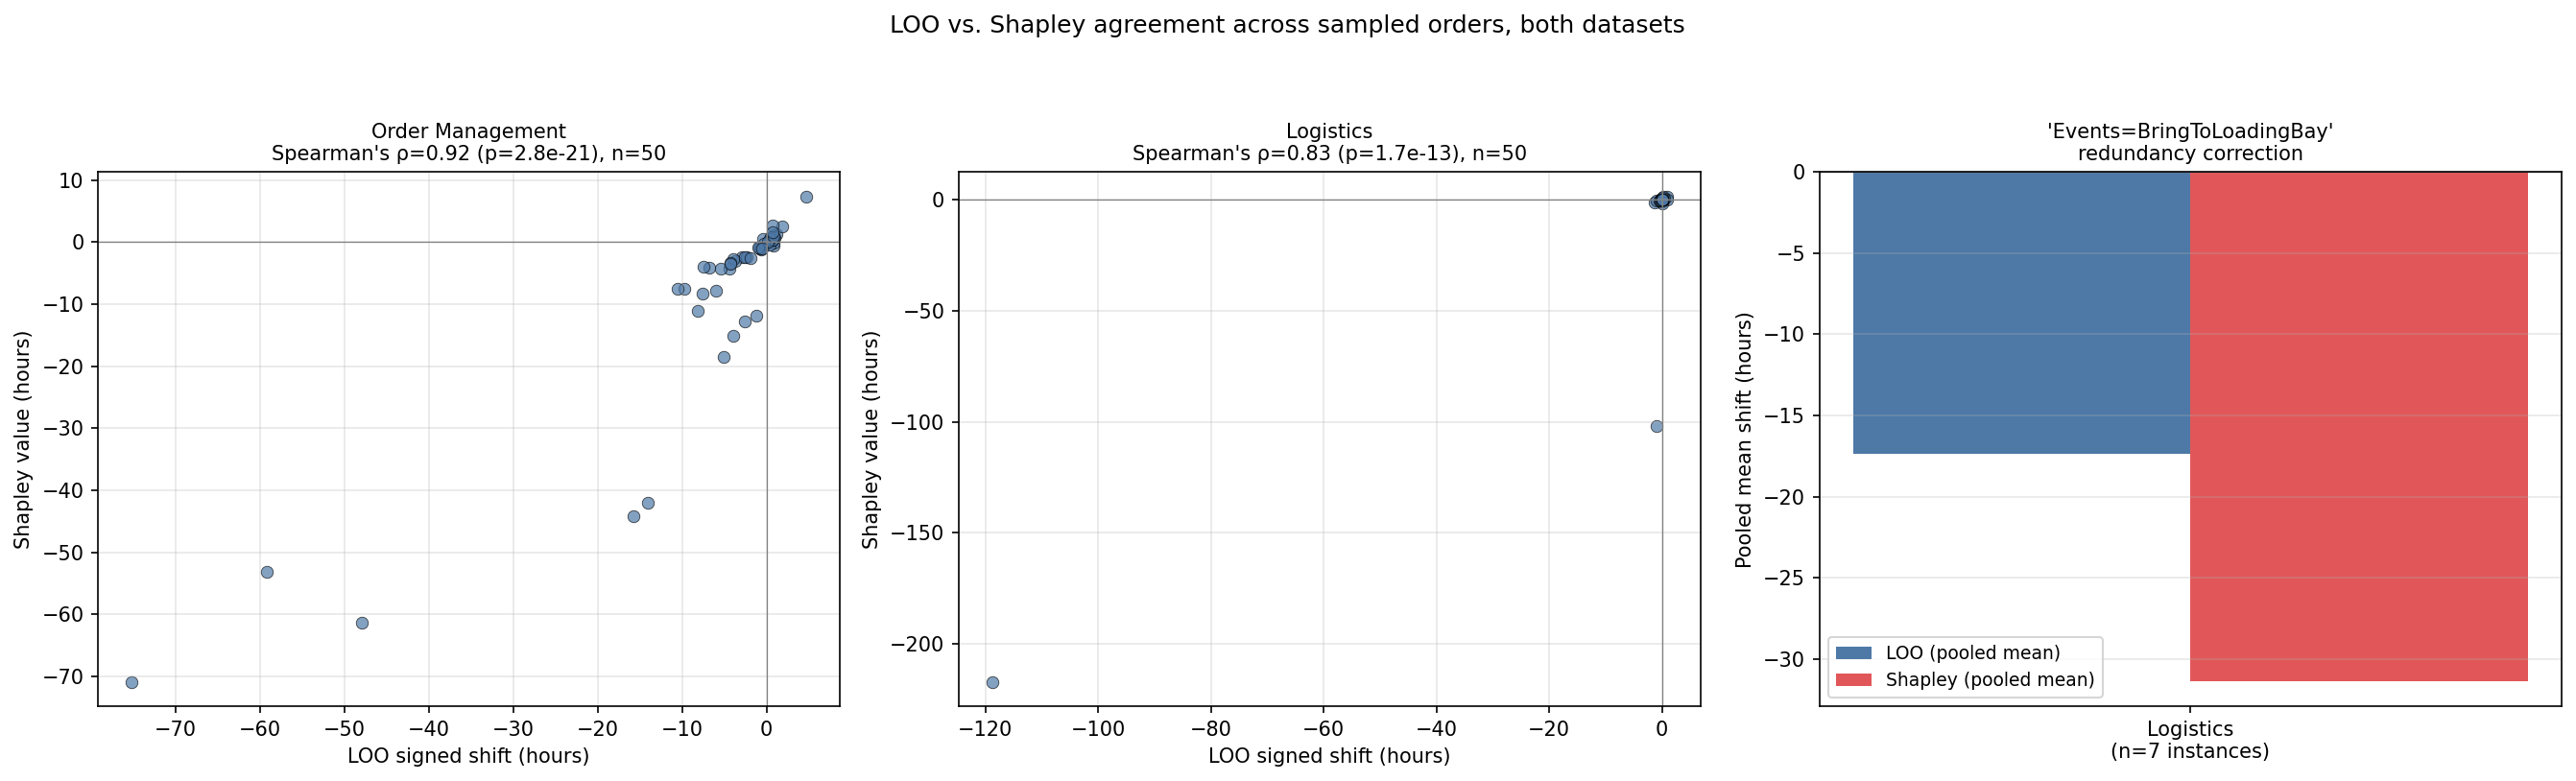
\includegraphics[width=1\textwidth]{figures/loo_vs_shapley_agreement.png}
                \caption{Measure of agreement between LOO method and full Shapley Values}
                \label{fig:loo_shapley_comp}
            \end{figure}
            
			Additionally, I needed to validate LOO's effectiveness as a proper identifier to limit the space over which Shapley Values would need to be run. Fig. \ref{fig:loo_shapley_comp} shows the result of this analysis. Both datasets show a strong, statistically significant rank agreement between the values identified by the two methods: Order Management reported a Spearman's $\rho$ value of 0.92 (p=2.8e-21), and Logistics reported a value of 0.83 (p=1.7e-13), each over 50 sampled orders. Despite this strong agreement in ranking, the two methods can still disagree on an element's exact magnitude when its underlying occurrences are redundant with one another. Logistics' \texttt{BringToLoadingBay} event, which recurs multiple times within a single process execution, illustrates this: LOO's pooled mean shift across the 7 instances where it appears is -17.3 hours, while Shapley's coalition-based accounting attributes -31.3 hours to the same event, correcting for the redundancy between its repeated occurrences that LOO's one-at-a-time removal underestimates. This highlights the continued need for Shapley Values as a proper quantifying method even where LOO's ranking alone is a reliable and much cheaper identifier.

            \begin{figure}[t!]
                \centering
                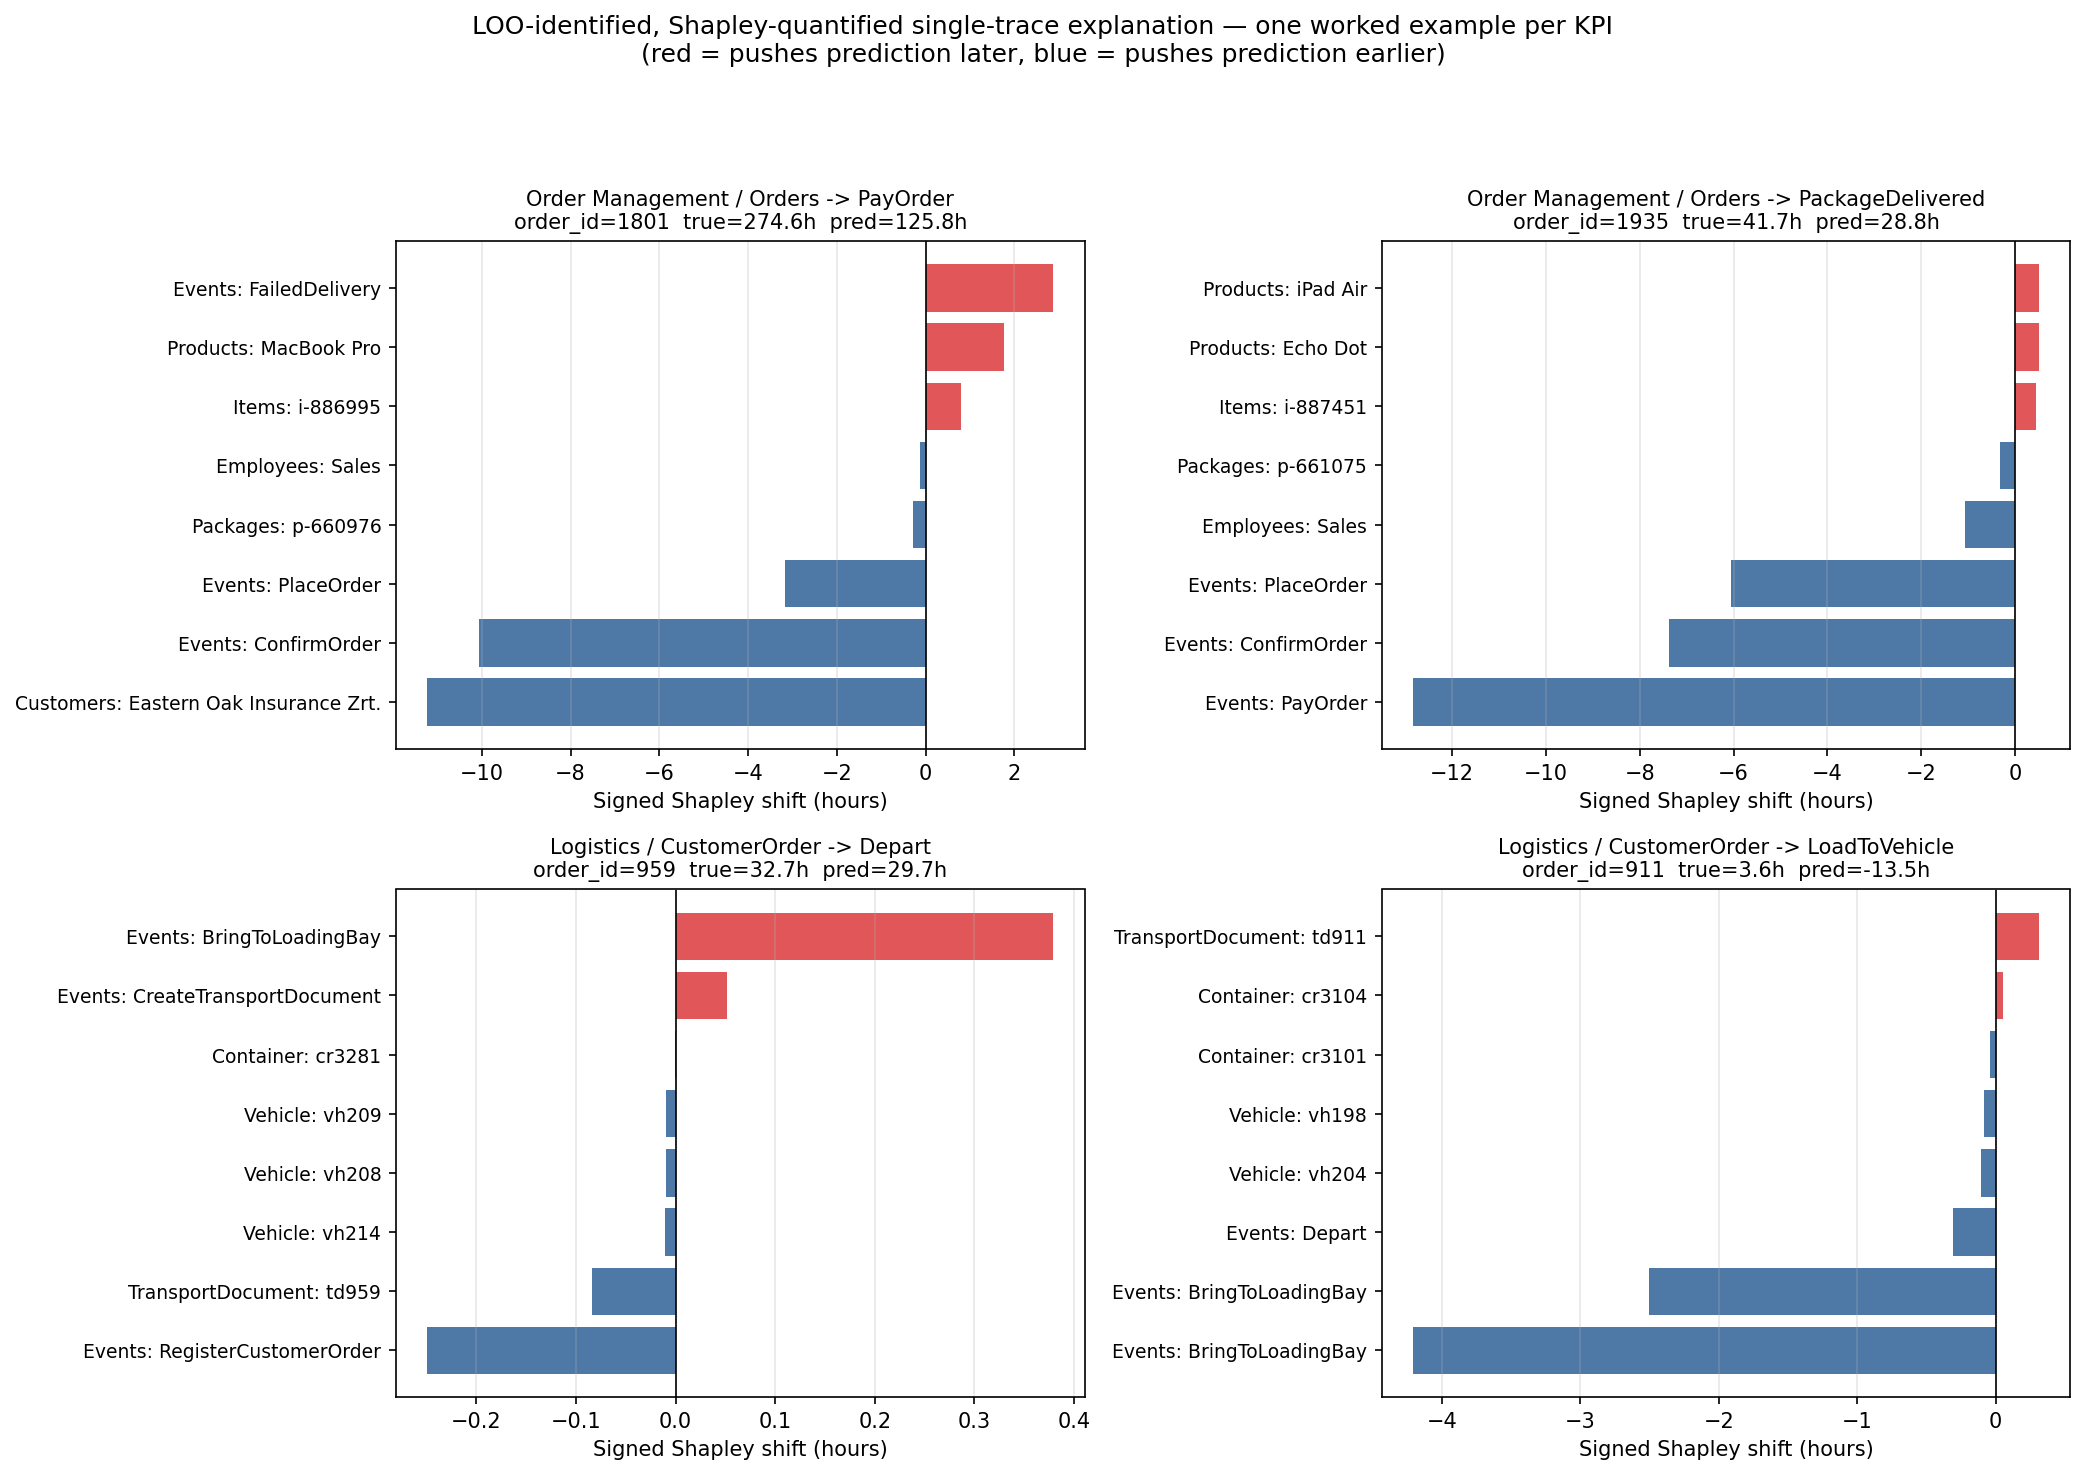
\includegraphics[width=1\textwidth]{figures/loo_shapley_trace_showcase.png}
                \caption{Graphs showing the single-trace explanations generated indicating the most important nodes in each trace as well as the impact on the model's prediction.}
                \label{fig:loo_shapley_showcase}
            \end{figure}

            \begin{figure}[t!]
                \centering
                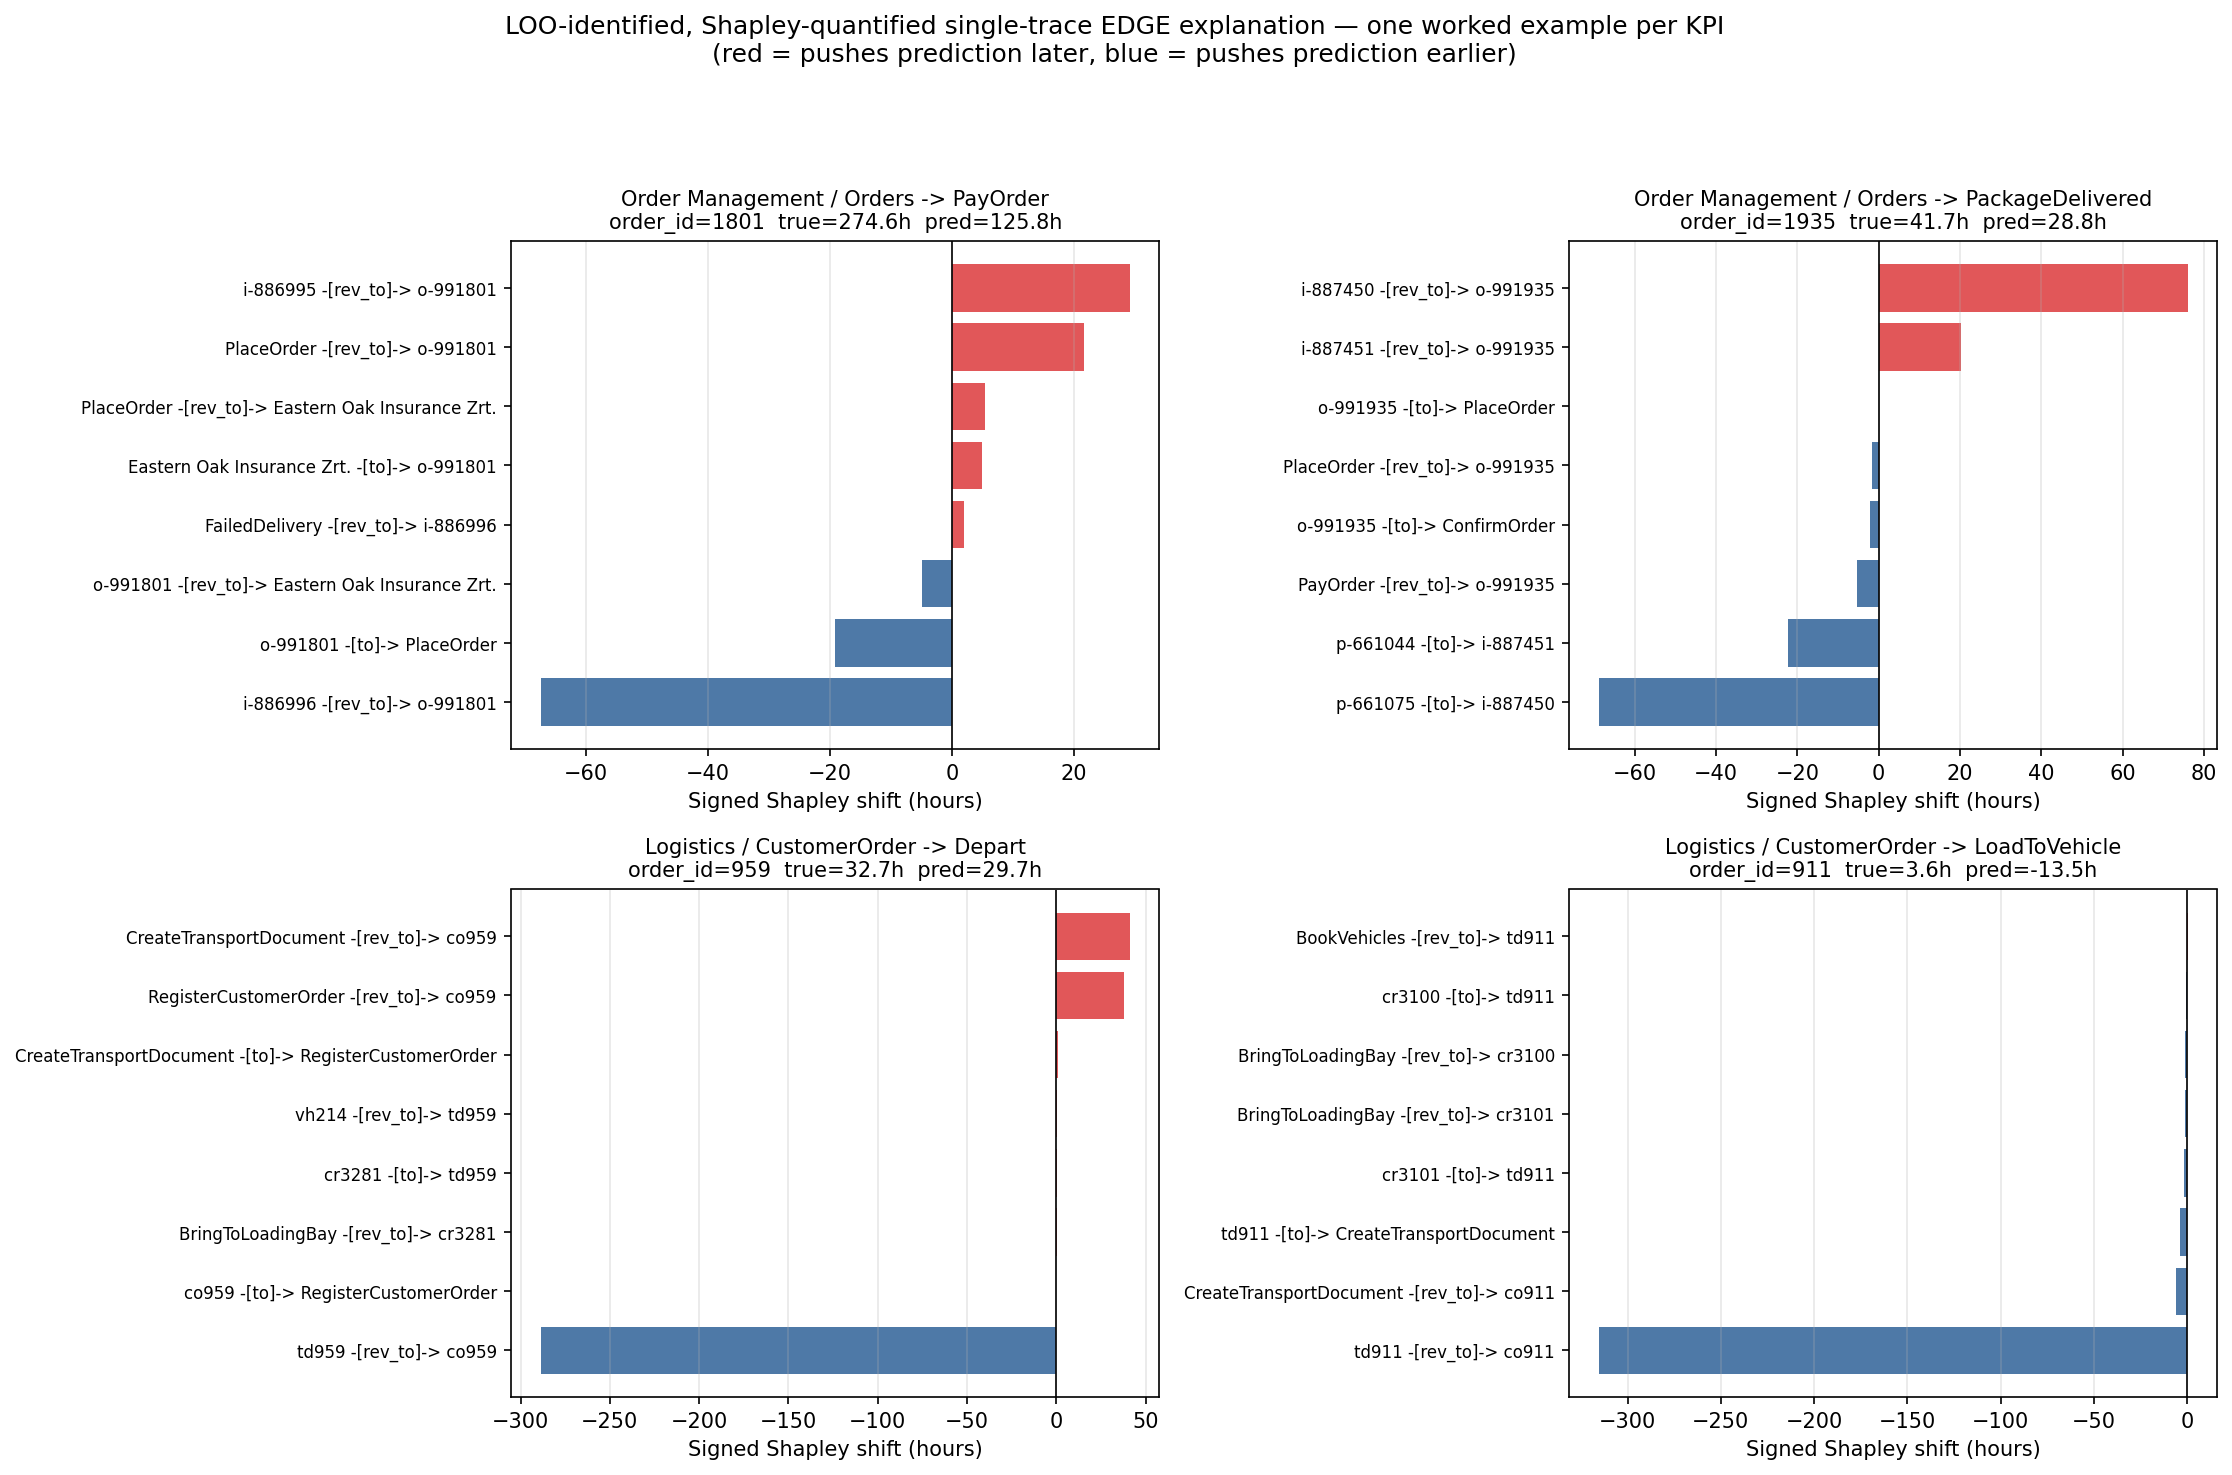
\includegraphics[width=1\textwidth]{figures/loo_shapley_edge_trace_showcase.png}
                \caption{Graphs showing the single-trace explanations generated indicating the most important edges in each trace as well as the impact on the model's prediction.}
                \label{fig:loo_edge_showcase}
            \end{figure}
            
            Before working through these examples, it is worth being explicit about how the single trace shown in them was chosen. Every single-trace figure in this section, as well as the gradient-based and counterfactual explanations shown later in this chapter, reuses the same order (order 1801, Order Management dataset, Orders $\to$ PayOrder) as one running example, rather than a fresh trace per figure. This is a deliberate choice made for narrative continuity, not a claim that the trace is representative: order 1801 was originally selected via a "slow trace" heuristic (a trace from the bottom quintile by remaining time, chosen to make for an interesting worked example), with no accuracy or fidelity criterion involved in its selection, and its own explanation fidelity later in this chapter turns out to be below the dataset average rather than favorably cherry-picked (Fig. \ref{fig:fidelity_graph}, characterization 0.565 against an aggregate LOO characterization of 0.815, Fig. \ref{fig:loo_comparison}). The dataset-wide, representative picture instead comes from the holistic aggregate view at the end of this section (Figs. \ref{fig:agg_shapley_global_om_payorder}-\ref{fig:agg_shapley_global_logistics_loadtovehicle}), which pools hundreds of predictions rather than illustrating a single one.

            Fig. \ref{fig:loo_shapley_showcase} shows examples of the graphs shown to the stakeholder for the single trace perturbation-based explanation. As can be seen the provided graphs show the node type and it's associated OCEL identifier. The node's impact on the model's prediction is shown in terms of hours, a proper understandable magnitude the stakeholder can interpret, with bar size and color showing the magnitude of the impact and its sign respectively, All this elements are considered in order to make the presented explanation as easily interpretable as possible by a stakeholder with limited knowledge about the workings of the predictive model. Additionally, the stakeholder is also provided with a table that gives a more structured view of the same information as the graphs.
			The presented analysis is applied to the three components of the input graph (nodes, edges and their associated feature values), each graph and table providing a summary of the information for each of these elements. Fig. \ref{fig:loo_edge_showcase} shows the same explanation process applied to the edges of prefixes in each dataset.

            \begin{figure}[t!]
                \centering
                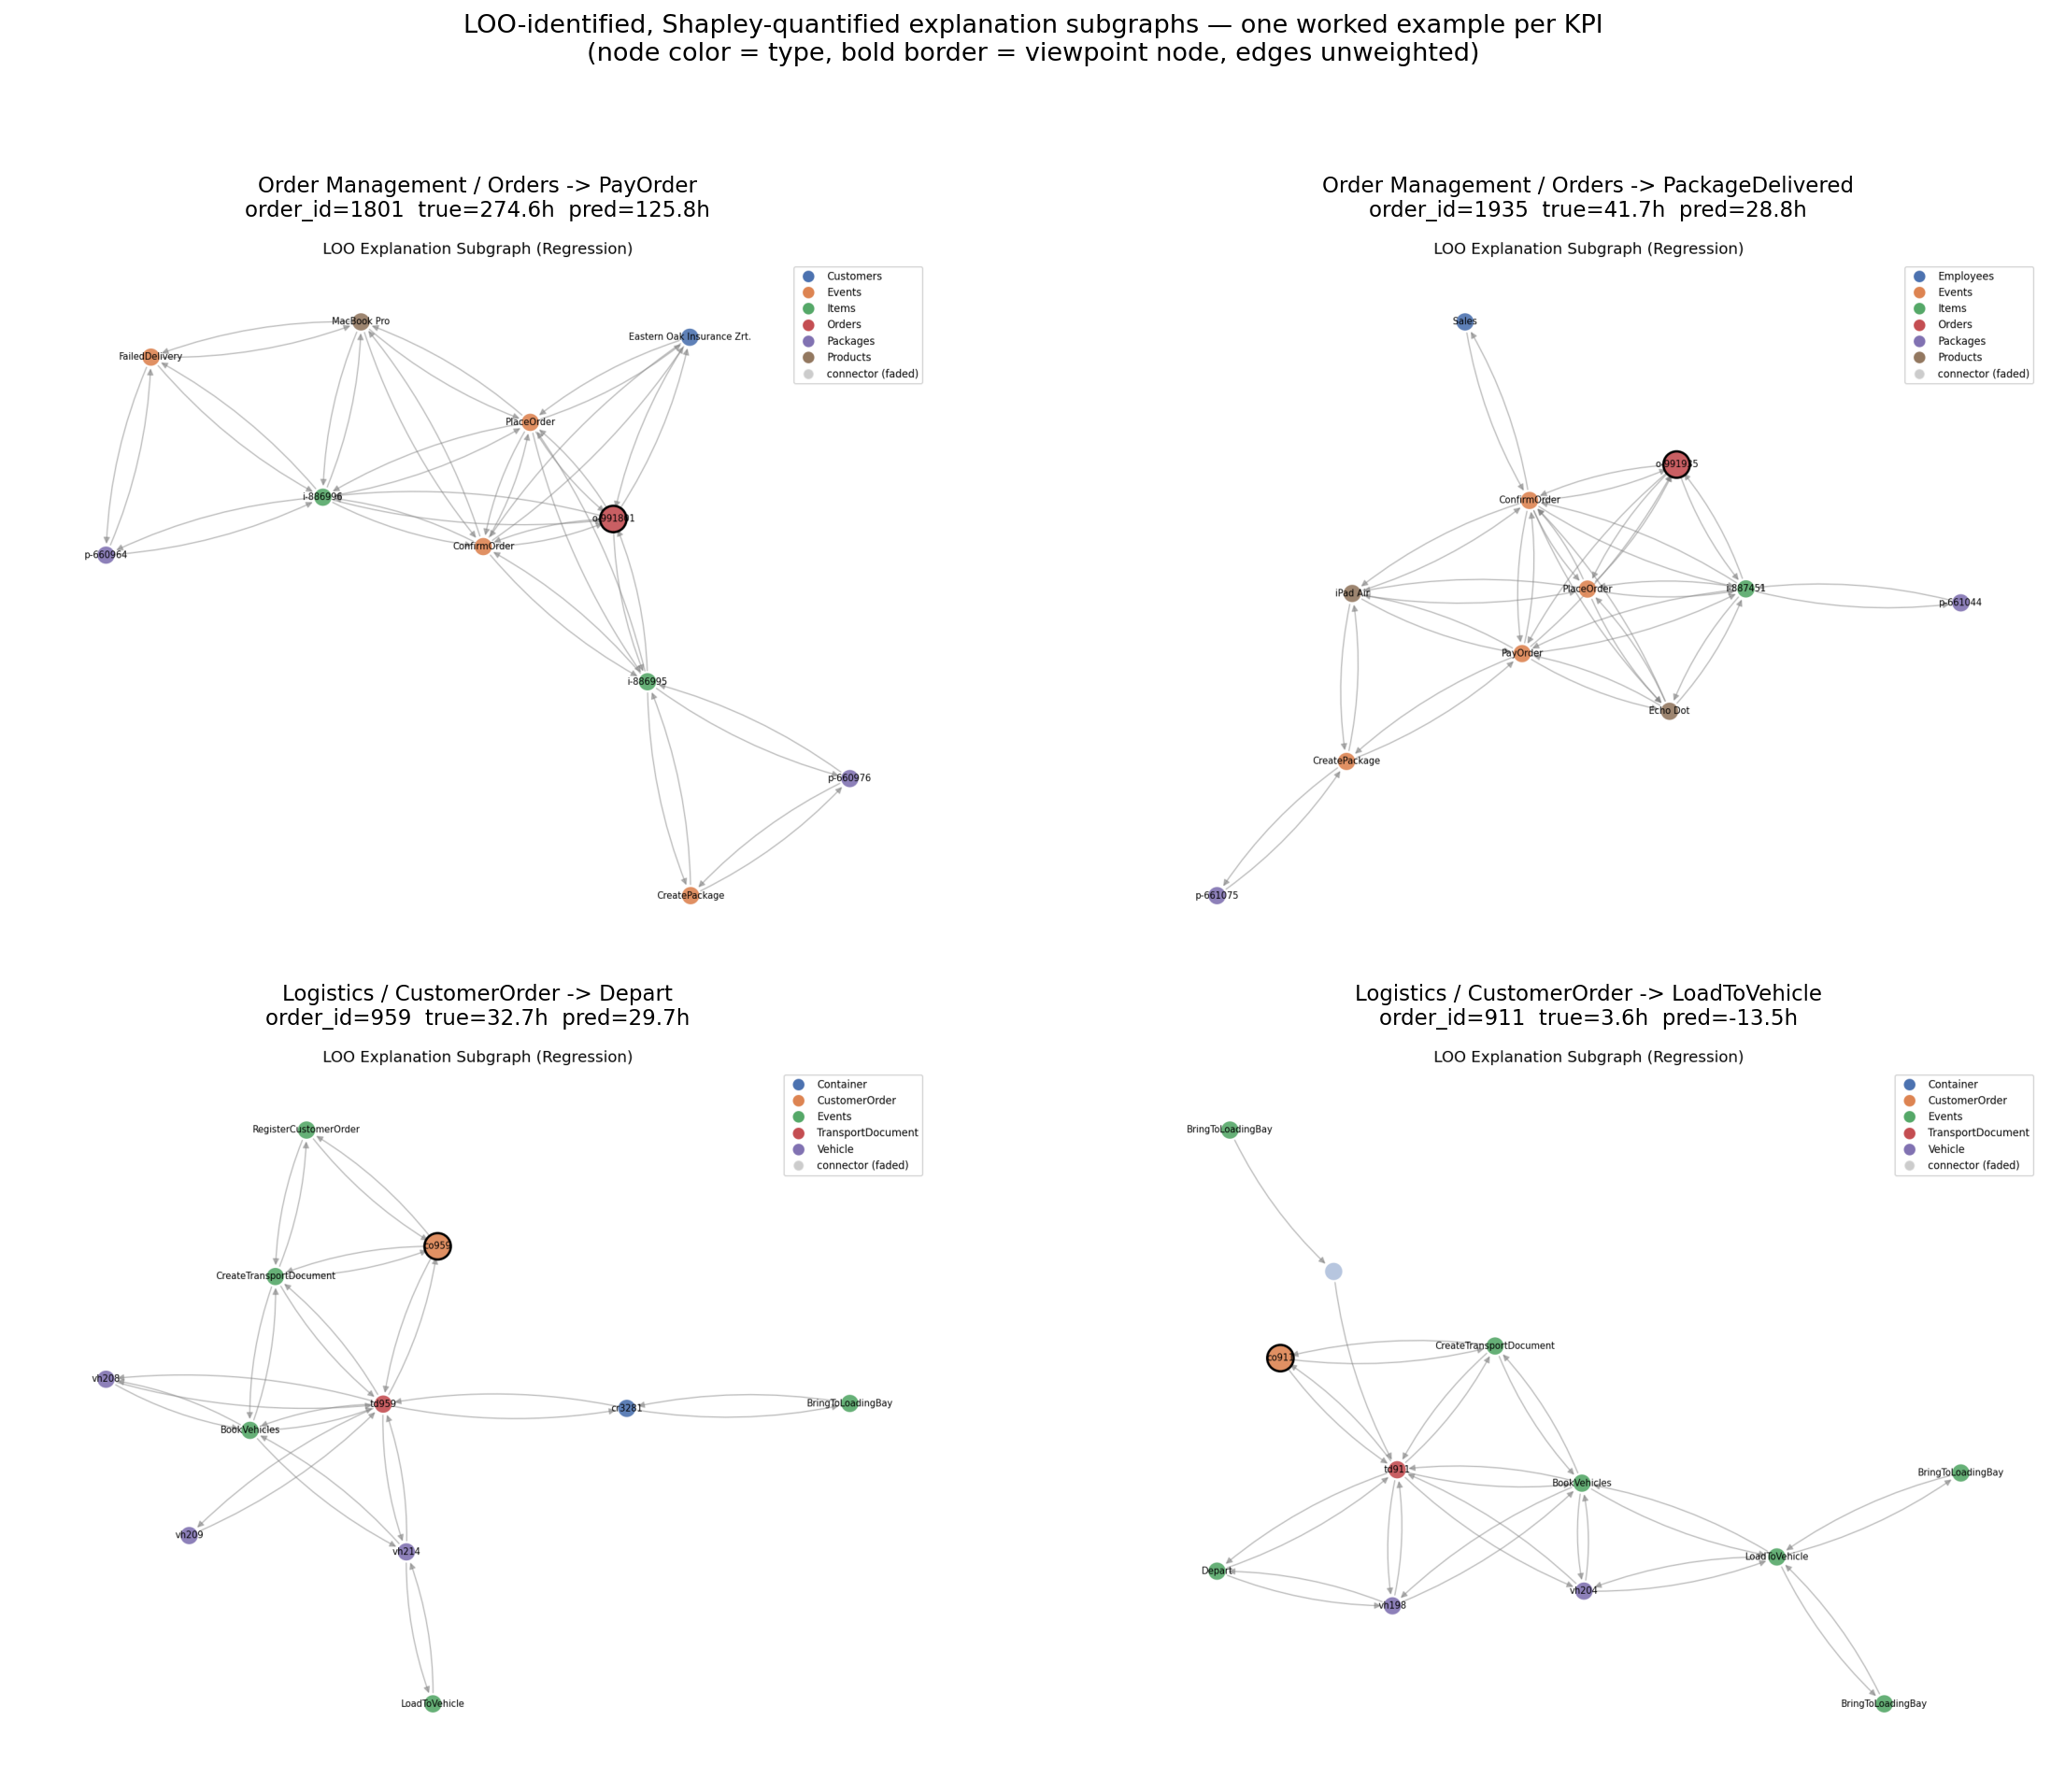
\includegraphics[width=1\textwidth]{figures/single_subgraph.png}
                \caption{Explanation subgraphs created using the identified most important nodes and edges, one worked example per KPI.}
                \label{fig:subgraph}
            \end{figure}
            
            Additionally, the end user is also provided with a visualization of the explanation subgraph created by the explanation. As can be seen in Fig. \ref{fig:subgraph} the subgraph is composed only of the most important elements identified by the explanation and provides another visual way of understanding the most impactful components of the process execution the model looked at when performing its prediction. In other words, the provided subgraph acts as a visual summary of the most impactful components of the input graph.

            \begin{figure}[t!]
                \centering
                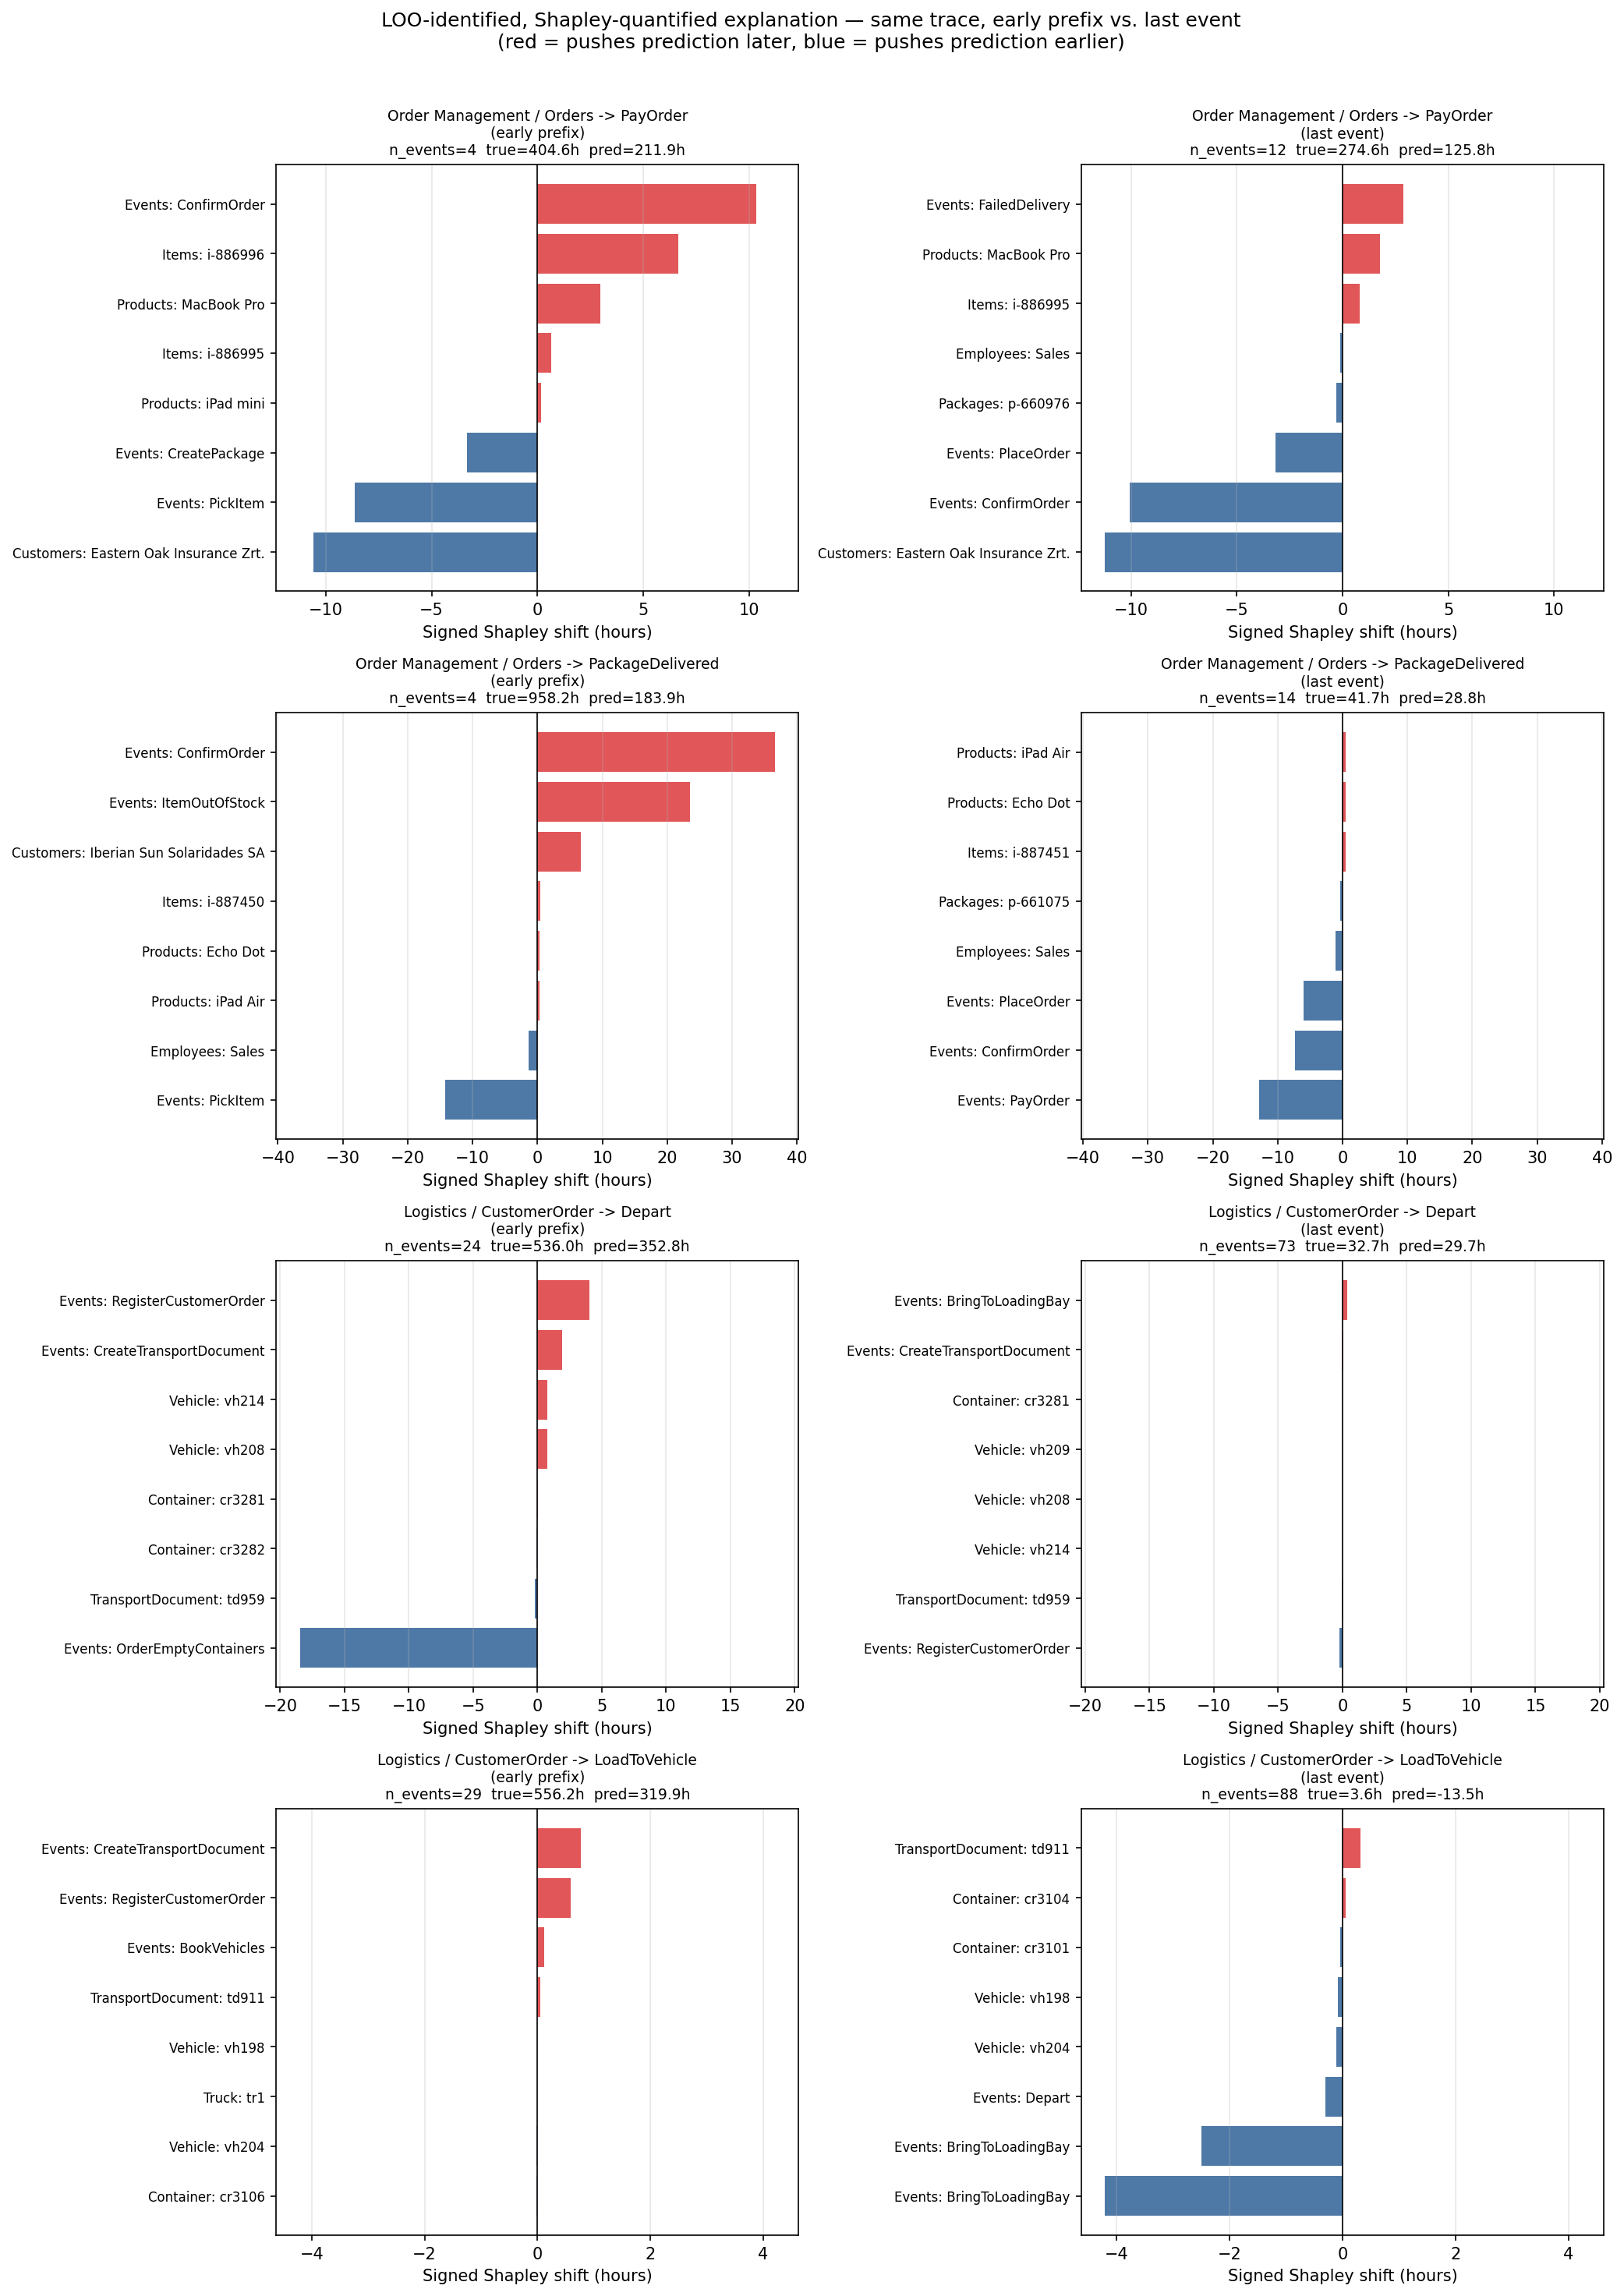
\includegraphics[width=0.85\textwidth]{figures/prefix_evolution.png}
                \caption{Graphs showing the single-trace explanations of node importance generated for an early prefix and the last-event prefix of the same process execution, for each of the four KPIs.}
                \label{fig:prefix_showcase}
            \end{figure}

			Fig. \ref{fig:prefix_showcase} shows that the given explanation can be applied to any prefix in a chosen process execution, giving the stakeholder the ability to view how the importance of elements shifts as the process moves along and more information is provided to the model. As can be seen in the figure, the ranking of important elements changes between the early prefix and the last-event prefix for every KPI shown -- for example, on the Order Management / Orders $\to$ PayOrder KPI, \texttt{ConfirmOrder} is the dominant positive driver on the early prefix but becomes a negative driver by the last event -- highlighting a shift in the model's understanding of the data provided as more information becomes available.
            
            \begin{figure}[t!]
                \centering
                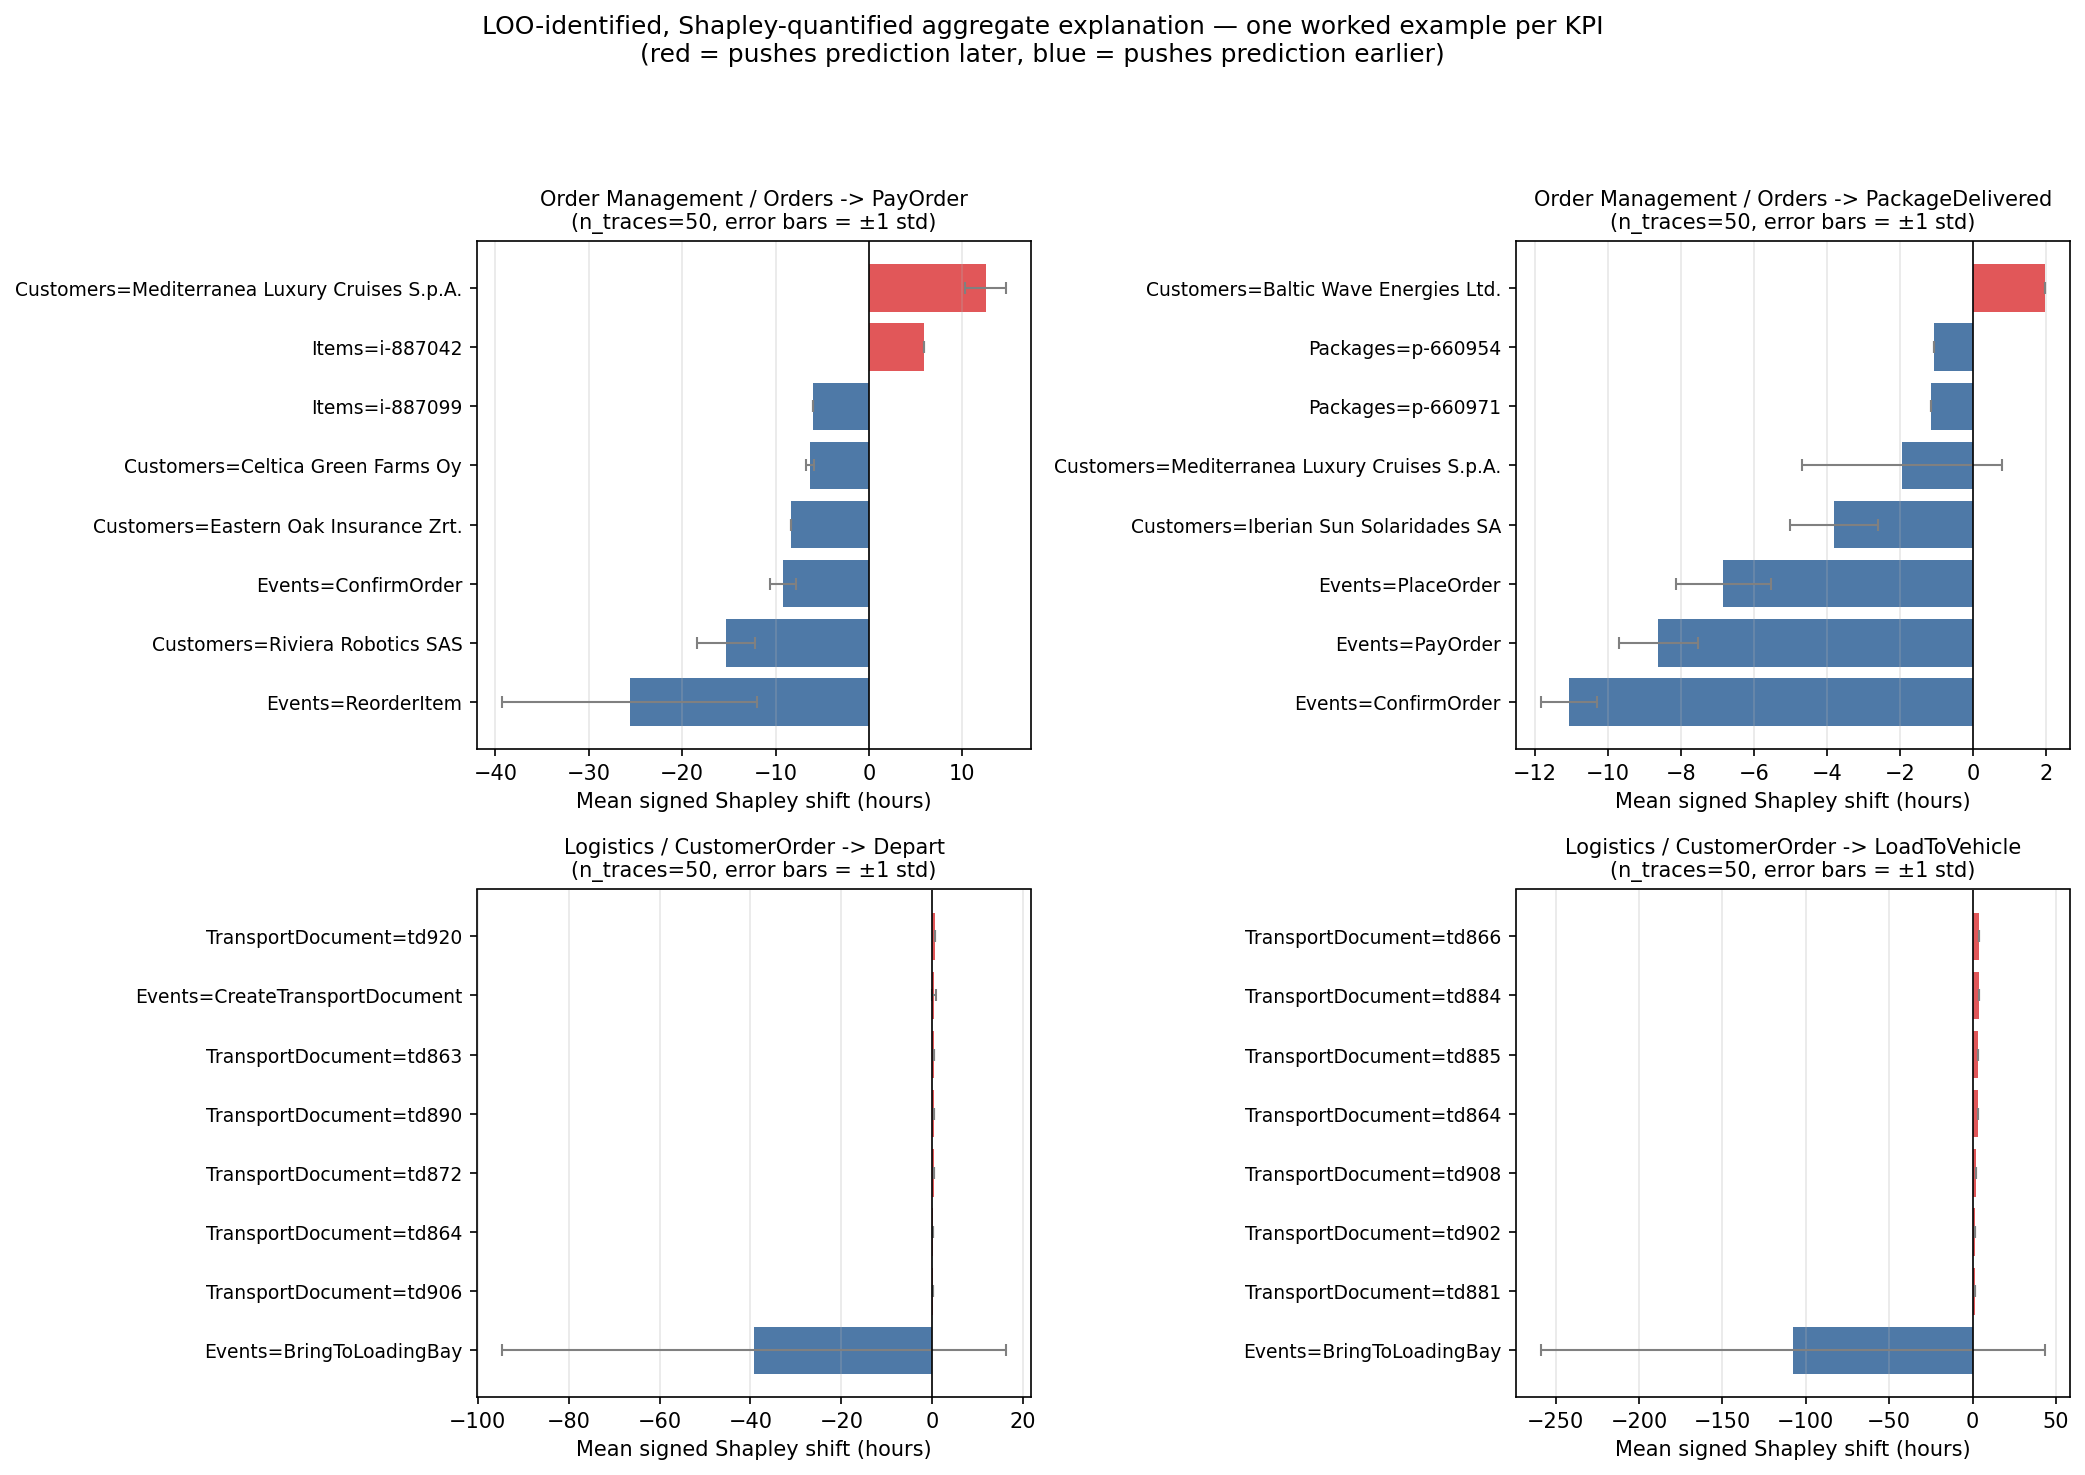
\includegraphics[width=1\textwidth]{figures/loo_shapley_aggregate_showcase.png}
                \caption{Graphs showing the aggregate explanations generated indicating the most important nodes for a collection of 50 traces as well as the impact on the model's prediction.}
                \label{fig:agg_shapley_showcase}
            \end{figure}

            Aside from single traces the stakeholder is also provided with an explanation over an aggregate set of traces. Fig. \ref{fig:agg_shapley_showcase} shows an example of the graphs provided measuring the impact of different node types on the model's prediction. The graphs give a rundown of the most important features of a given type (nodes, edges and their associated feature values) over the chosen universe of prefixes.
			In order to maintain cohesion within the presentation, each graph is designed to mirror its single trace counterpart.

            \subsubsection{Holistic aggregate view}
            \begin{figure}[t!]
                \centering
                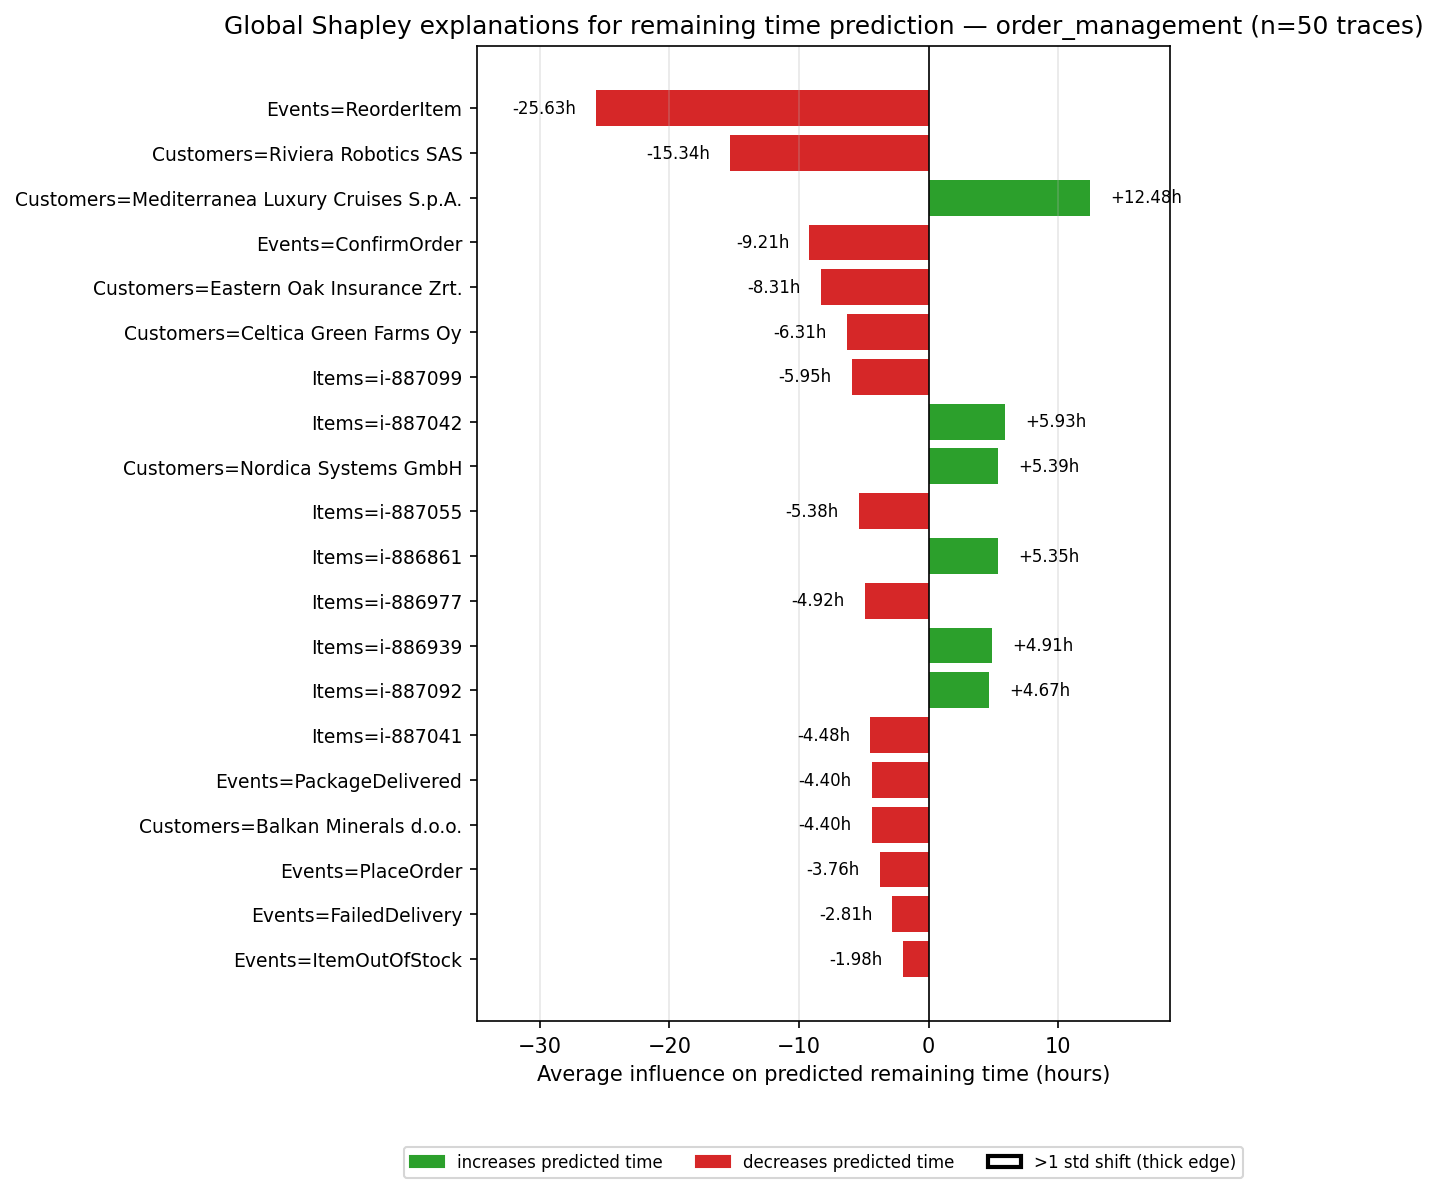
\includegraphics[width=1\textwidth]{figures/aggregate_shapley_global_om_payorder.png}
                \caption{Global LOO+Shapley explanation, ranked across all identified elements, for Order Management / Orders $\to$ PayOrder (50 traces).}
                \label{fig:agg_shapley_global_om_payorder}
            \end{figure}

            \begin{figure}[t!]
                \centering
                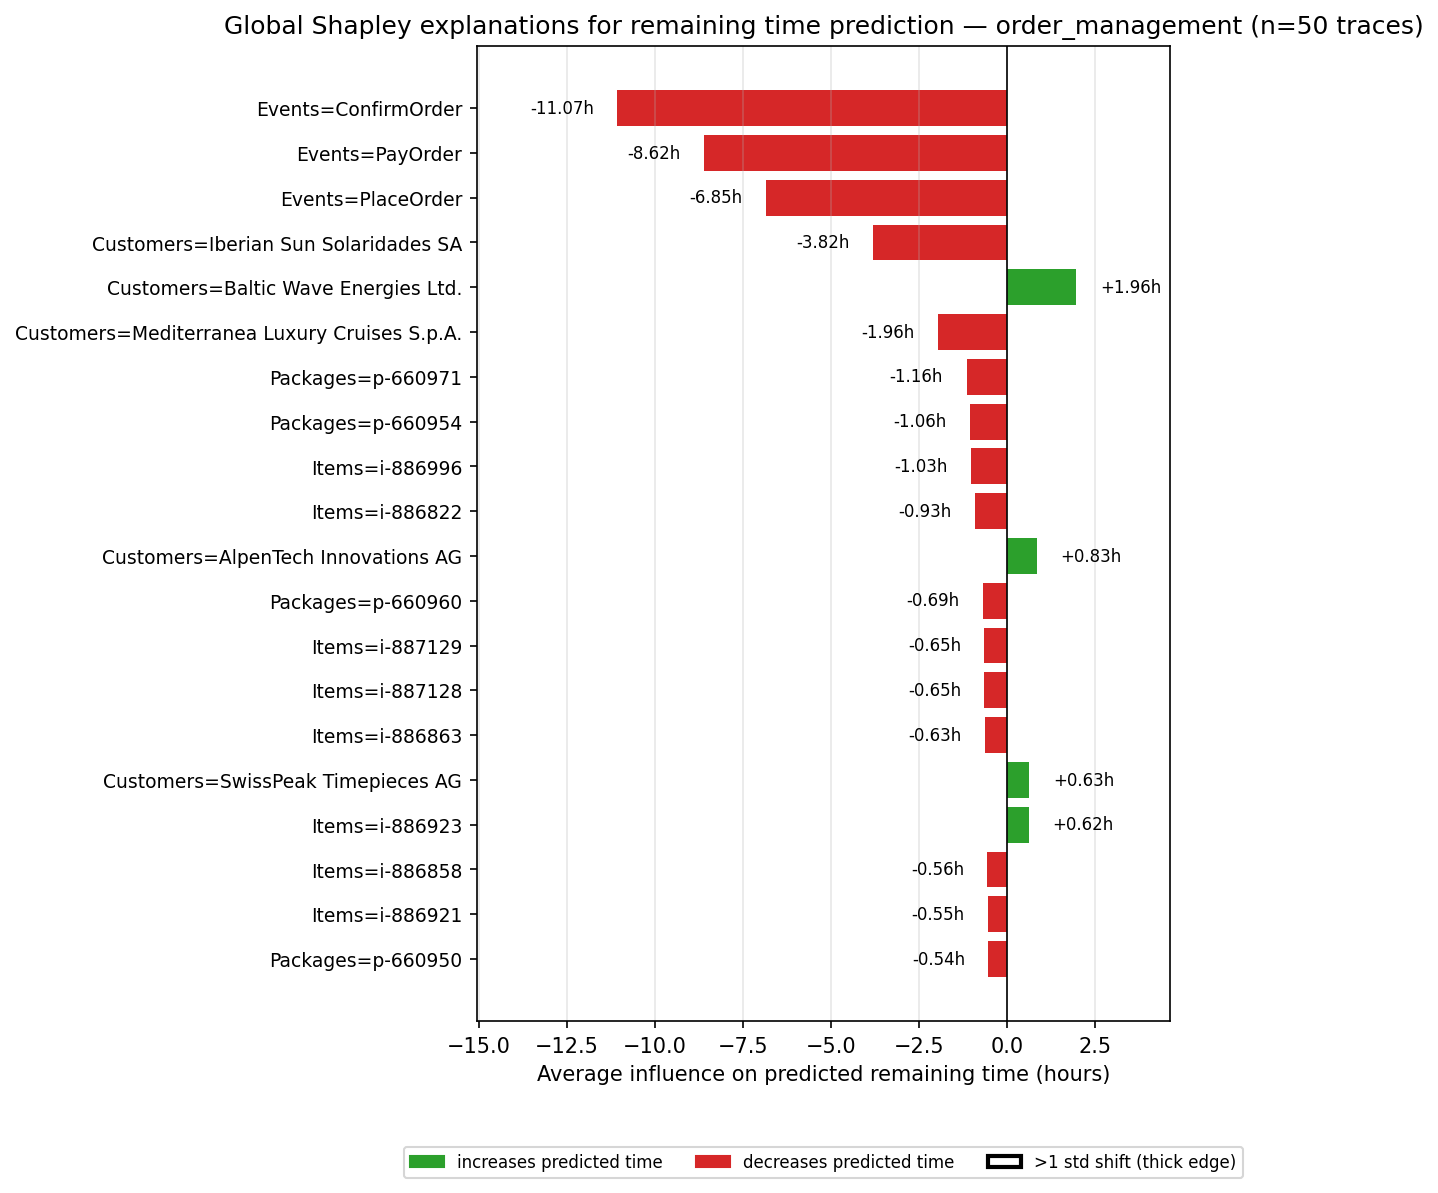
\includegraphics[width=1\textwidth]{figures/aggregate_shapley_global_om_packagedelivered.png}
                \caption{Global LOO+Shapley explanation, ranked across all identified elements, for Order Management / Orders $\to$ PackageDelivered (50 traces).}
                \label{fig:agg_shapley_global_om_packagedelivered}
            \end{figure}

            \begin{figure}[t!]
                \centering
                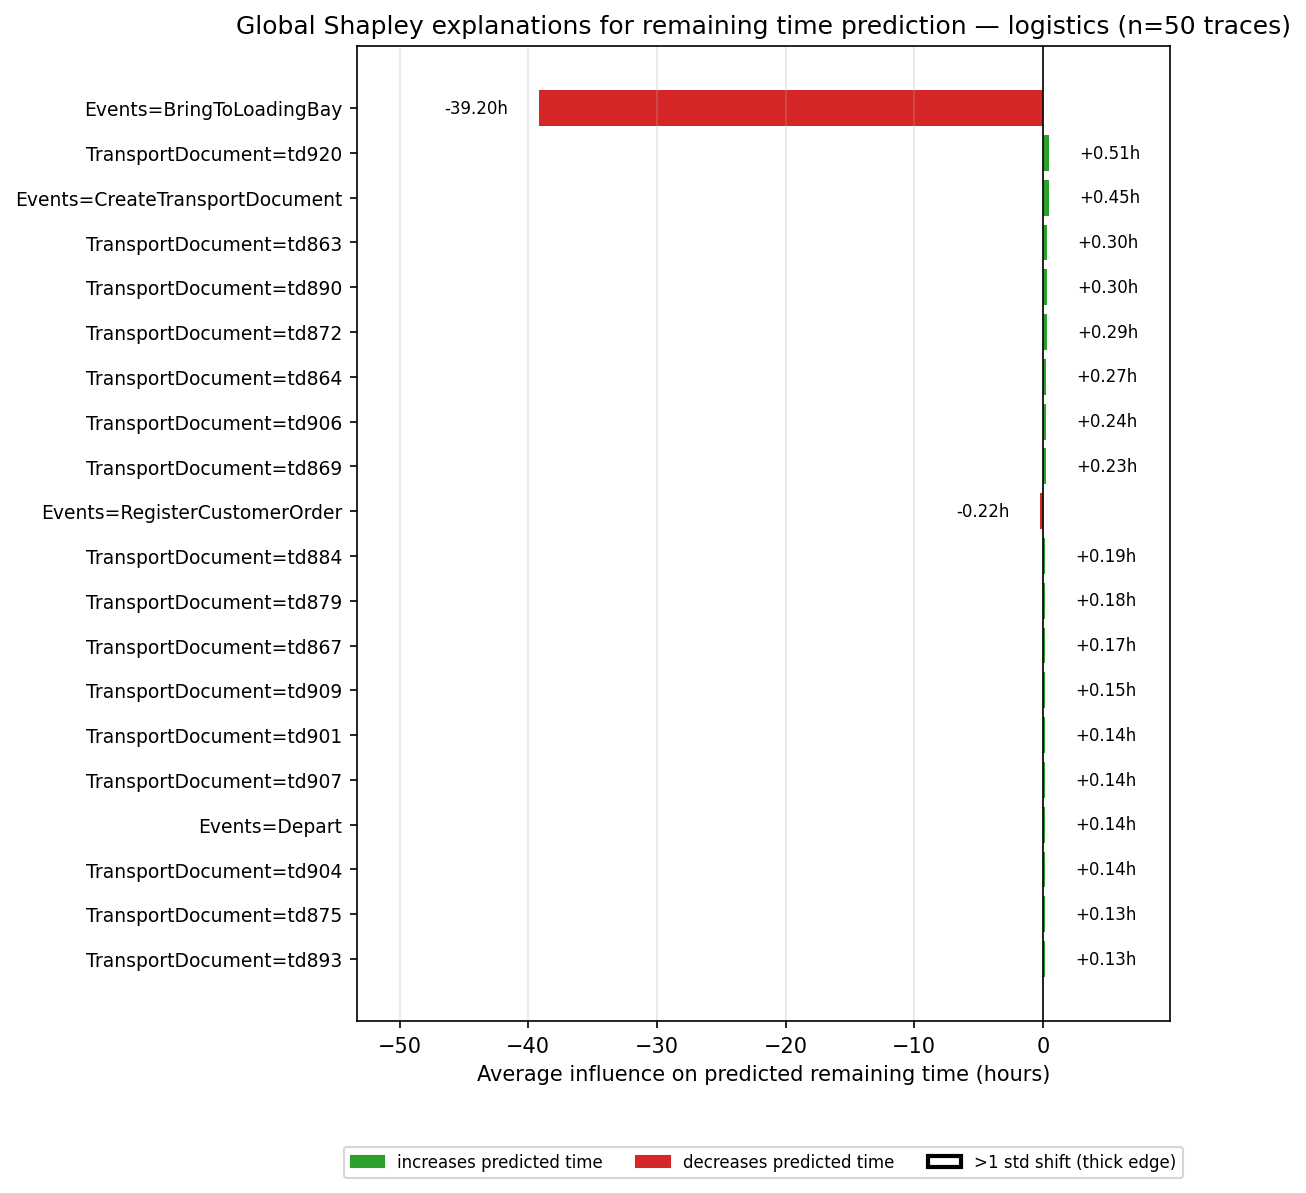
\includegraphics[width=1\textwidth]{figures/aggregate_shapley_global_logistics_depart.png}
                \caption{Global LOO+Shapley explanation, ranked across all identified elements, for Logistics / CustomerOrder $\to$ Depart (50 traces).}
                \label{fig:agg_shapley_global_logistics_depart}
            \end{figure}

            \begin{figure}[t!]
                \centering
                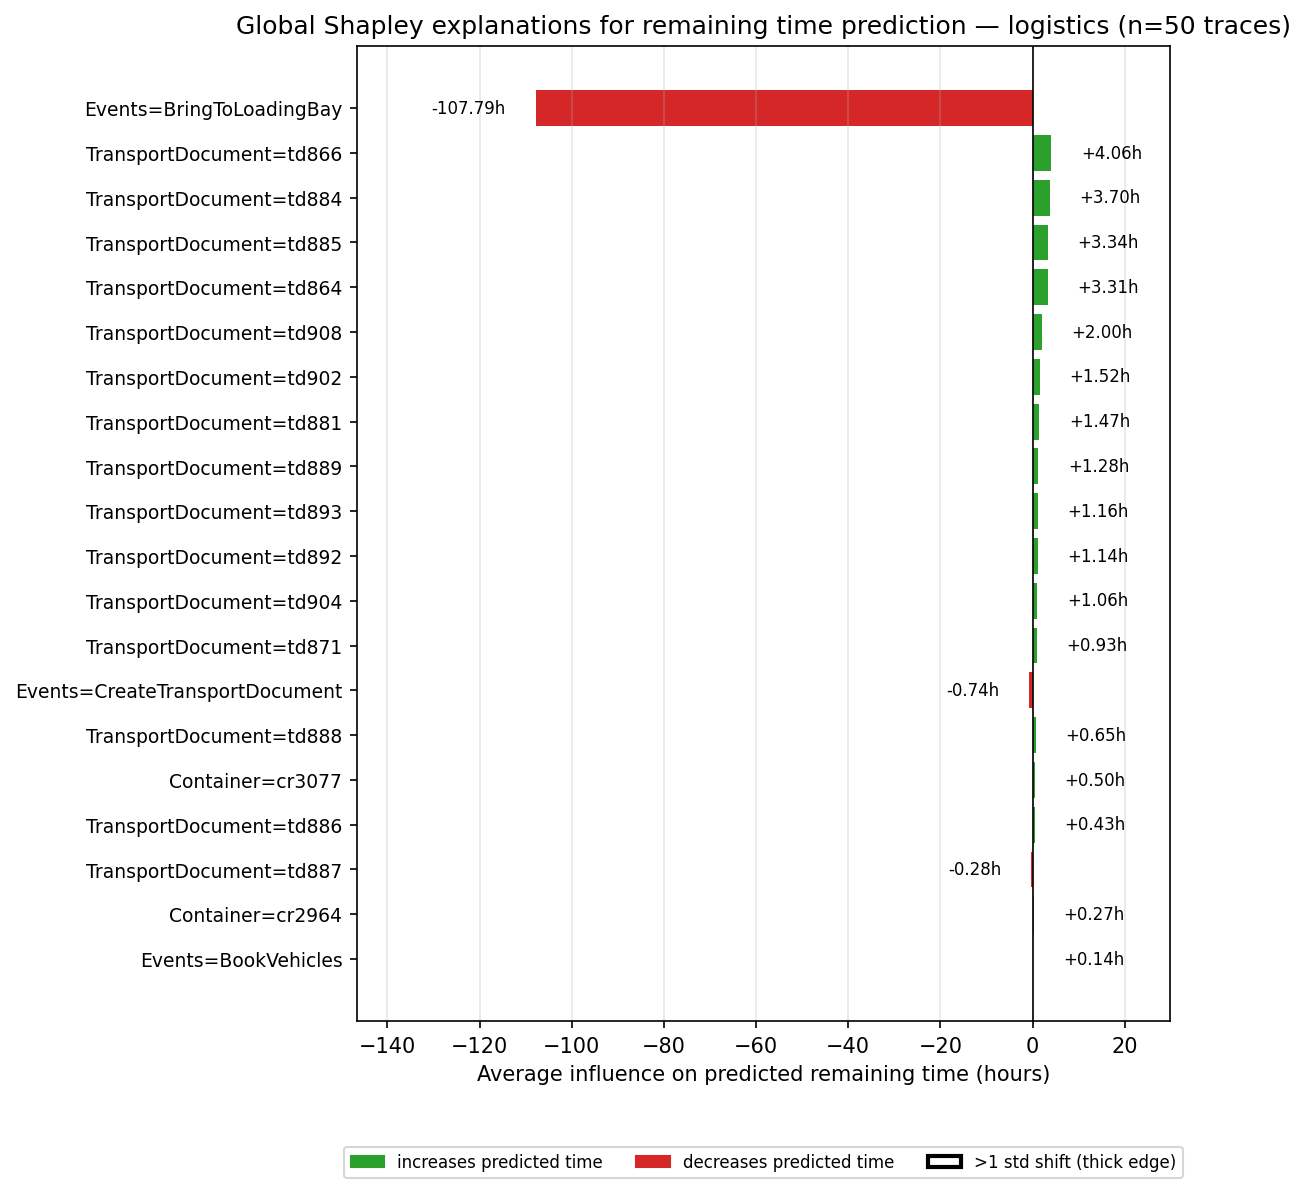
\includegraphics[width=1\textwidth]{figures/aggregate_shapley_global_logistics_loadtovehicle.png}
                \caption{Global LOO+Shapley explanation, ranked across all identified elements, for Logistics / CustomerOrder $\to$ LoadToVehicle (50 traces).}
                \label{fig:agg_shapley_global_logistics_loadtovehicle}
            \end{figure}

            The graphs shown so far in this section describe the \emph{quality} of the explanations -- how faithful they are (Fig. \ref{fig:loo_comparison}), how consistent LOO is with full Shapley Values (Fig. \ref{fig:loo_shapley_comp}) -- or, in Fig. \ref{fig:agg_shapley_showcase}'s case, a compact per-KPI summary limited to a handful of elements. None of them give a single, holistic view of what the framework identifies as important across the dataset as a whole. Figs. \ref{fig:agg_shapley_global_om_payorder}-\ref{fig:agg_shapley_global_logistics_loadtovehicle} close that gap: each is a single ranked list, pooled across the same 50 traces per KPI used elsewhere in this section, showing every node identity (event type, customer, item, package, transport document, etc.) whose presence shifted the model's prediction, signed and ranked by its average impact. Rather than illustrating one trace or comparing two methods, these graphs give the stakeholder a genuine ``helicopter view'' of the model's behavior as a whole: which recurring elements of the process consistently push predictions earlier or later, independent of any single example.

        \subsection{Gradient/feature-based explanation}
            \begin{figure}[t!]
                \centering
                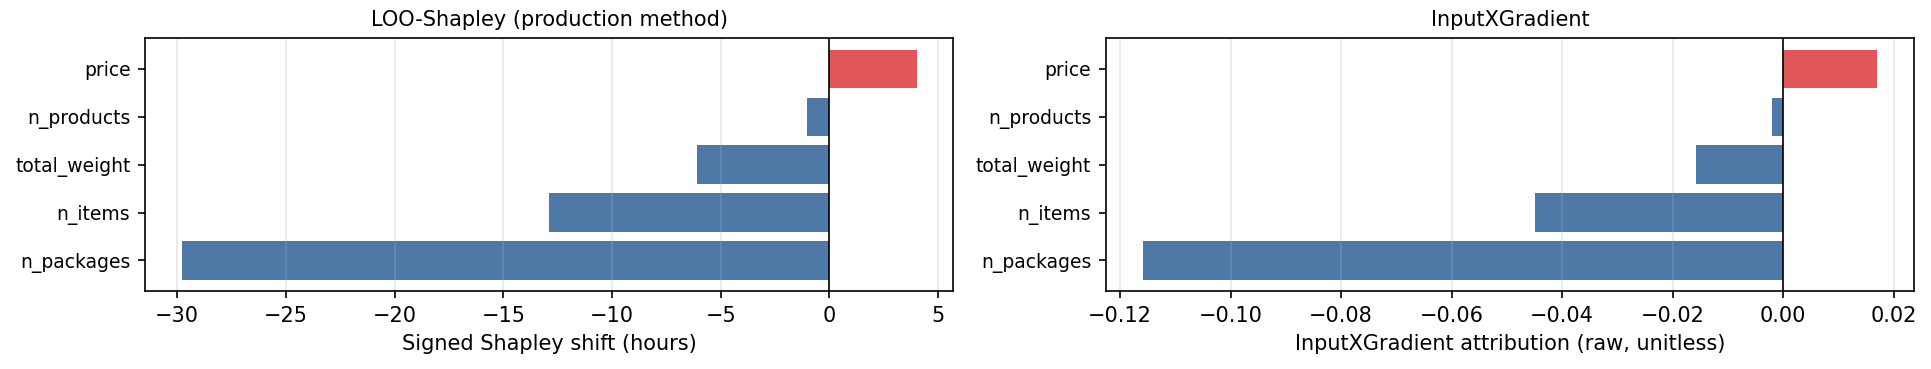
\includegraphics[width=1\textwidth]{figures/gradient_shapley_comparison_inputxgradient.png}
                \caption{Graphs showing the single-trace explanation provided for feature importance on the Order node using the Gradient $\cdot$ Input method for identification and the LOO-Shapley method for quantifying the feature's impact on the prediction.}
                \label{fig:input_gradient}
            \end{figure}

            \begin{figure}[t!]
                \centering
                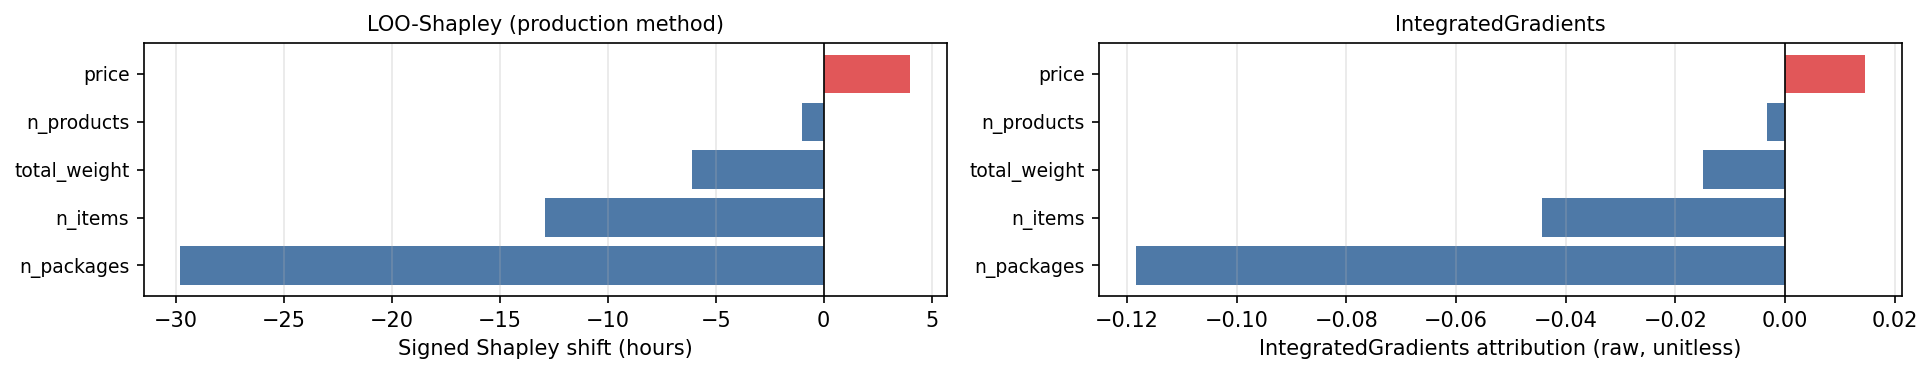
\includegraphics[width=1\textwidth]{figures/gradient_shapley_comparison_integratedgradients.png}
                \caption{Graphs showing the single-trace explanation provided for feature importance on the Order node using the Integrated Gradients method for identification and the LOO-Shapley method for quantifying the feature's impact on the prediction.}
                \label{fig:integ_gradients}
            \end{figure}
            
            While node and edge importance are calculated exclusively through the use of the perturbation-based method their associated feature values follow a different methodology. Fig. \ref{fig:input_gradient} and Fig. \ref{fig:integ_gradients} show the ranking of feature importance for the feature values present in a given trace for the Orders node. The values presented in the right side graph of Fig. \ref{fig:input_gradient} refer to the attribution values calculated through the chosen gradient-based explanation method, in this case Gradient $\cdot$ Input. In order to present this value in a quantifiable way the stakeholder is also shown a graph such as the one in the left side. This graph provides the physical magnitude of the impact for each of the identified feature values from the first analysis. The graph follows the same design as the graphs shown for the other elements of the input graph in order to maintain cohesion in the presentation. Fig. \ref{fig:integ_gradients} showcases that the methodology allows the stakeholder to choose their desired feature attribution method if they wished to compare the rankings provided by each one.

            \begin{figure}[t!]
                \centering
                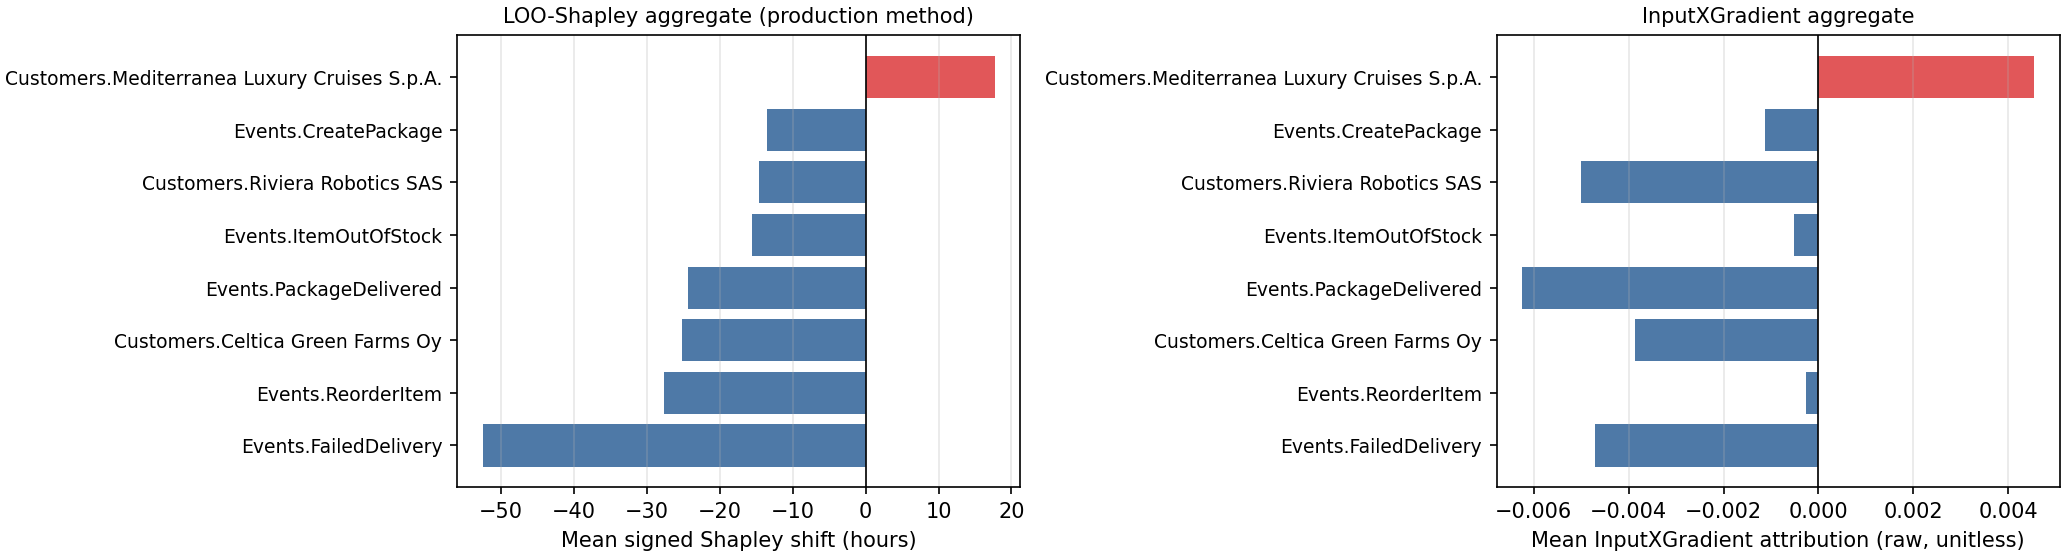
\includegraphics[width=1\textwidth]{figures/feature_attribution_aggregate_shapley_comparison_inputxgradient.png}
                \caption{Graphs showing the aggregate explanation provided for feature importance of the nodes in the chosen traces using the Gradients $\cdot$ Input method for identification and the LOO-Shapley method for quantifying the feature's impact on the prediction.}
                \label{fig:agg_input_gradients}
            \end{figure}

            \begin{figure}[t!]
                \centering
                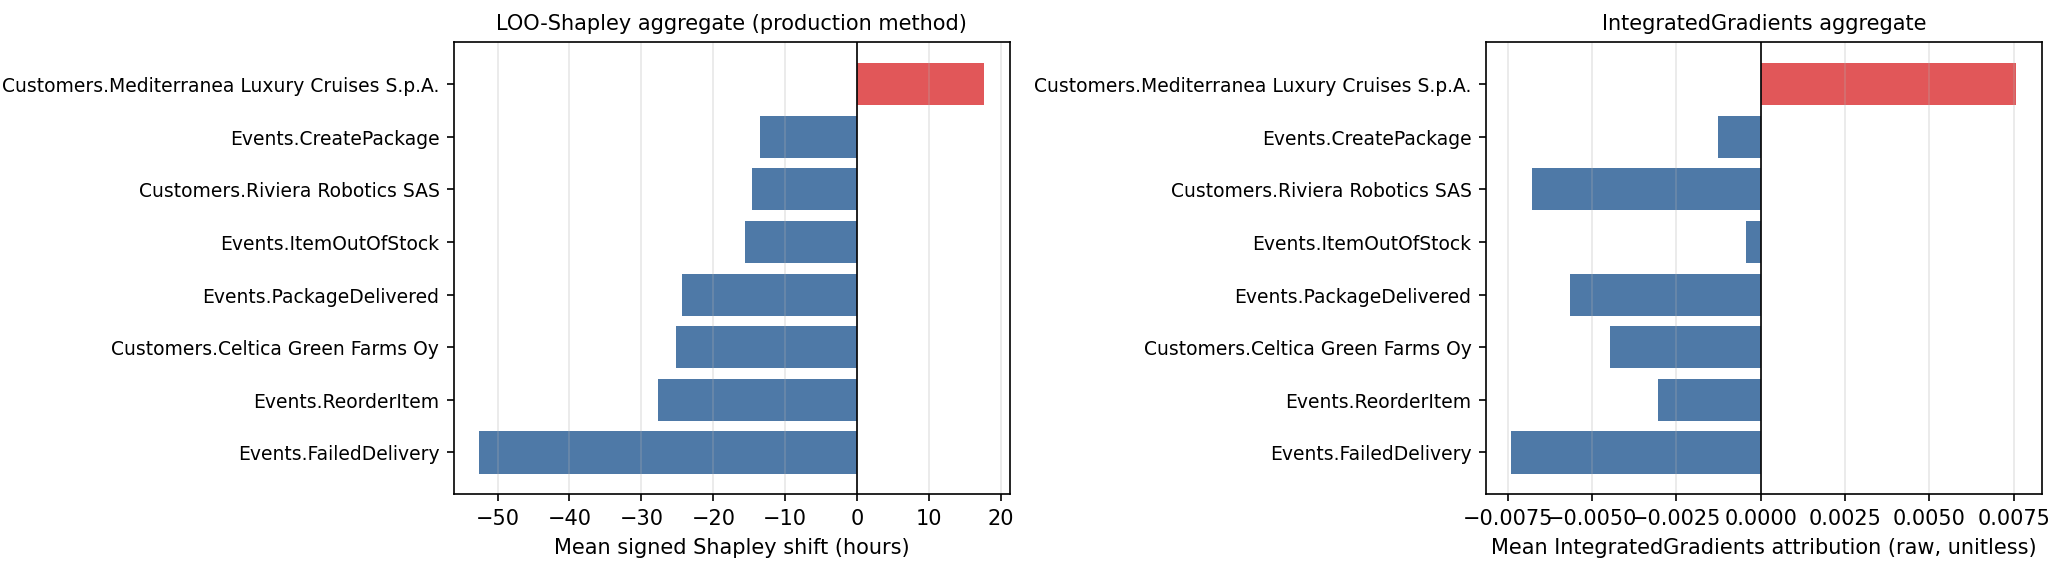
\includegraphics[width=1\textwidth]{figures/feature_attribution_aggregate_shapley_comparison_integratedgradients.png}
                \caption{Graphs showing the aggregate explanation provided for feature importance of the nodes in the chosen traces using the Integrated Gradients method for identification and the LOO-Shapley method for quantifying the feature's impact on the prediction.}
                \label{fig:agg_integ_gradients}
            \end{figure}
            
            In the same vein as the perturbation-based explanation, this method can also be applied to a collection of prefixes in an aggregate analysis. Fig. \ref{fig:agg_input_gradients} and Fig. \ref{fig:agg_integ_gradients} show the resulting graphs. Following the pattern shown for the first explanation, the stakeholder is presented with a graph that identifies the most impactful features of the nodes over the entire prefix set as well as the average impact their presence has on the model's predicted output. Same as with the single-trace analysis, the stakeholder is able to choose which gradient method they prefer to use for the explanation, allowing them to compare the results of each methodology.

        \subsection{Counterfactual explanation}
        \begin{figure}[t!]
                \centering
                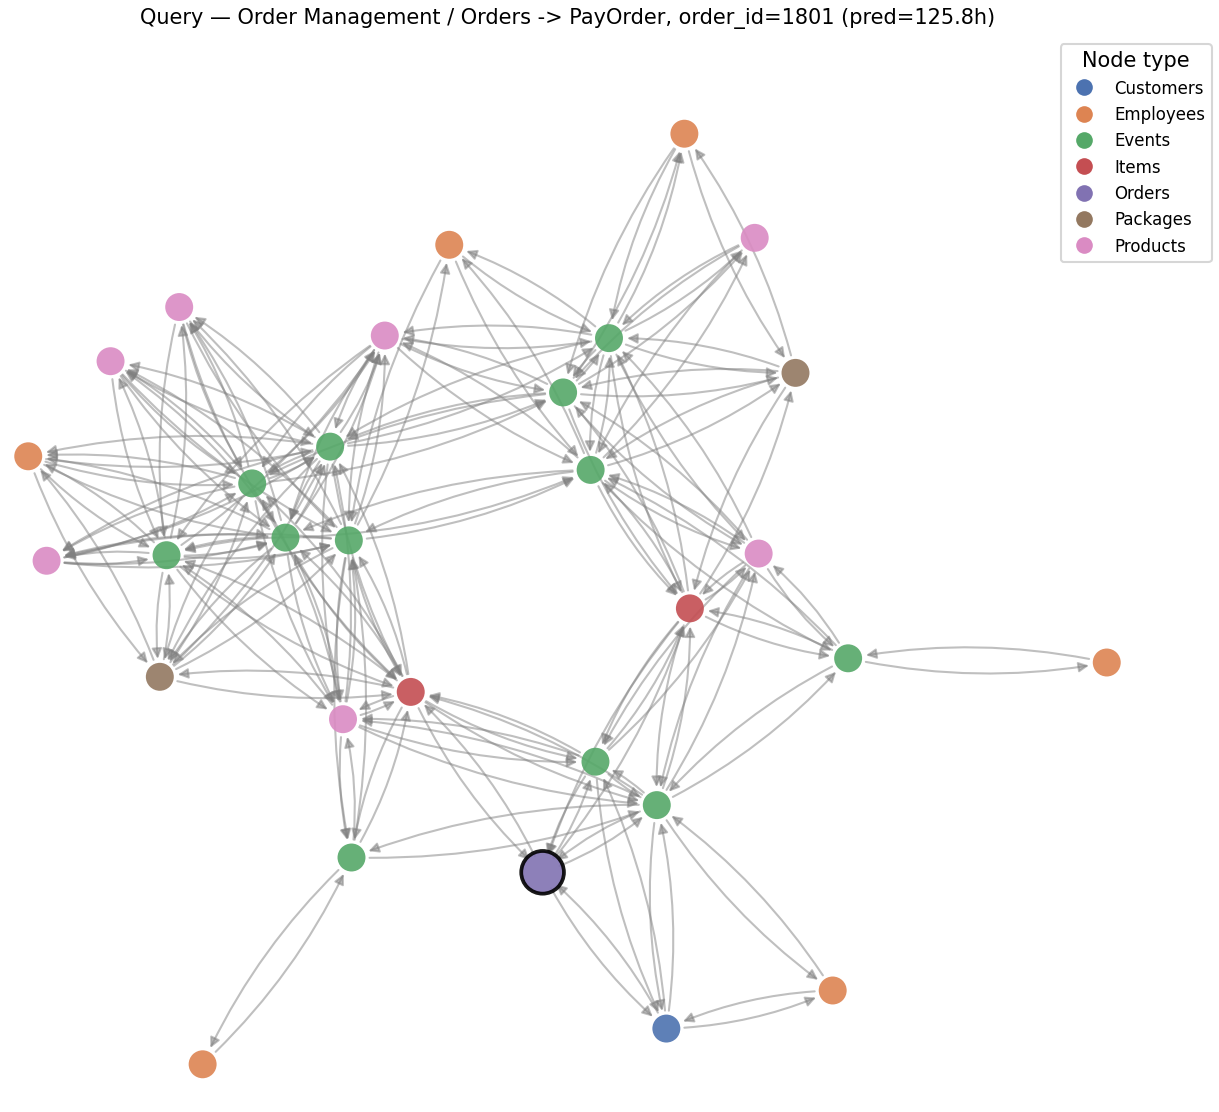
\includegraphics[width=1\textwidth]{figures/cf_showcase_query_graph.png}
                \caption{Graph representation of the user's selected graph for counterfactual explanation.}
                \label{fig:cf_query_graph}
            \end{figure}

        \begin{figure}[t!]
            \centering
            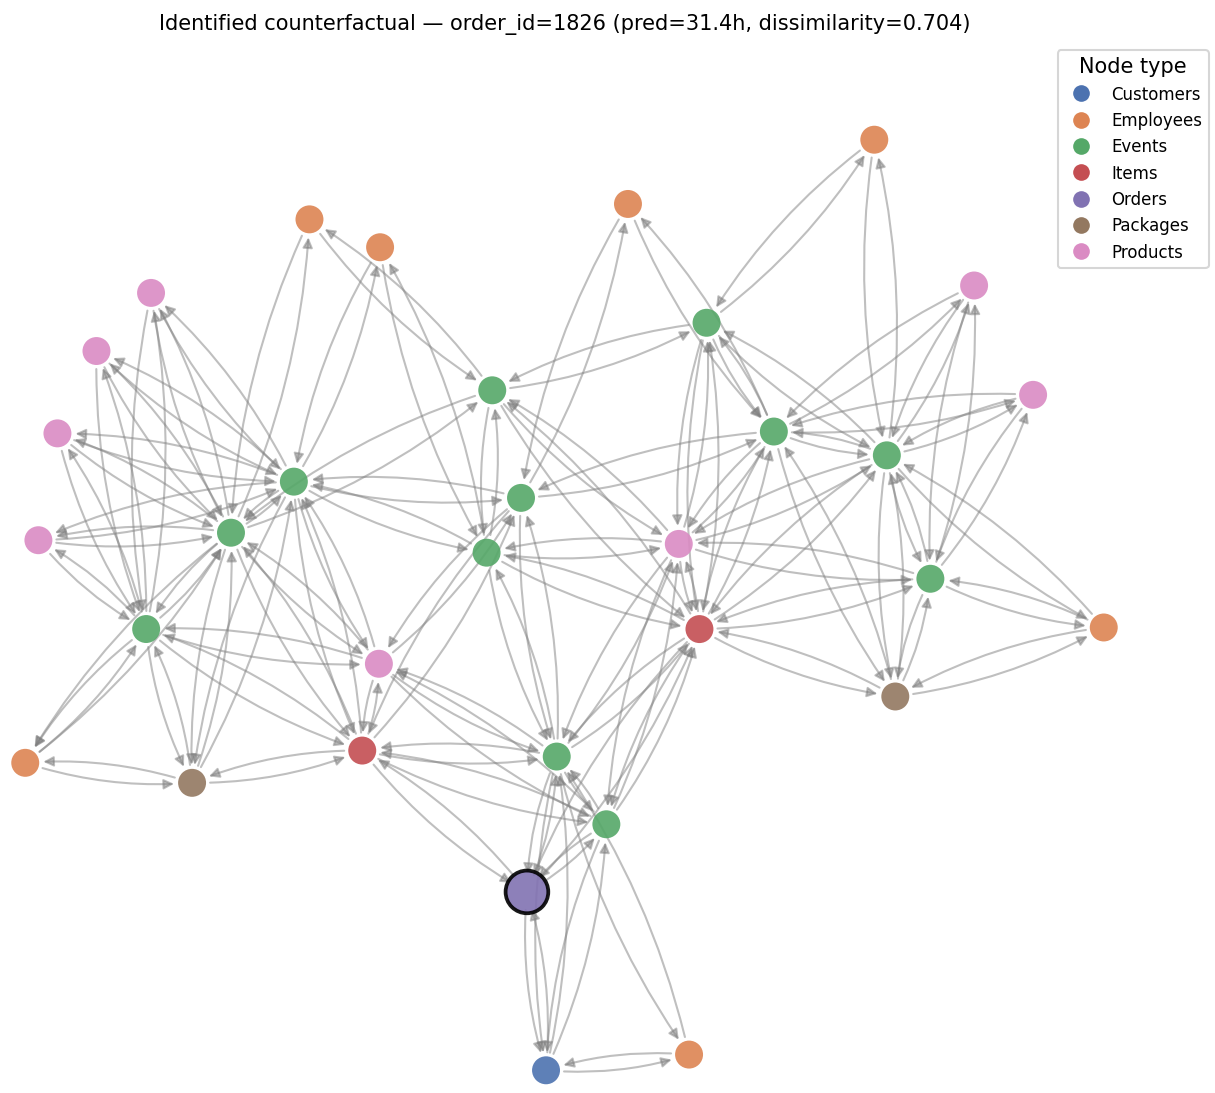
\includegraphics[width=1\textwidth]{figures/cf_showcase_counterfactual_graph.png}
            \caption{Graph representation of the counterfactual graph identified for counterfactual explanation.}
            \label{fig:cf_graph}
        \end{figure}

        \begin{figure}[t!]
            \centering
            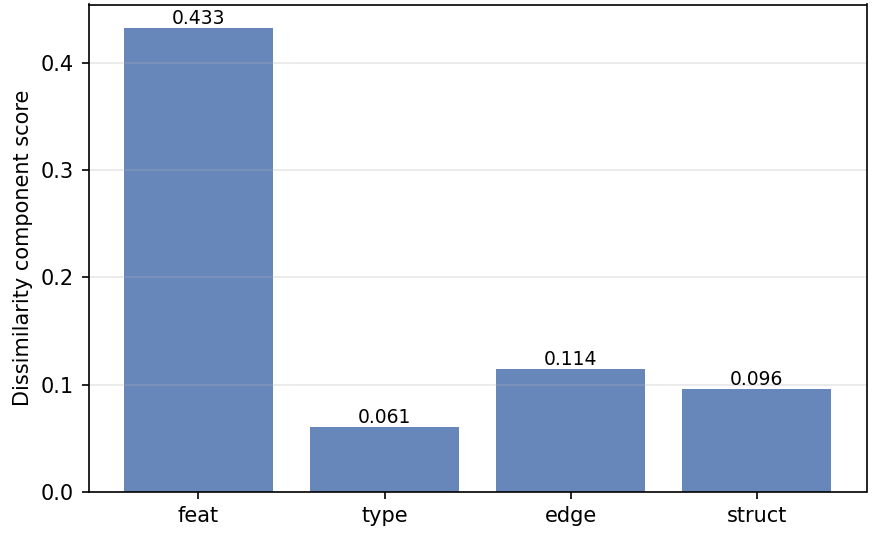
\includegraphics[width=1\textwidth]{figures/cf_showcase_dissimilarity_breakdown.png}
            \caption{Graph representation of the dissimilarity values for the distinct elements compared between the user's chosen graph and the chosen counterfactual.}
            \label{fig:cf_dissim_breakdown}
        \end{figure}
            
        My proposed counterfactual explanation relies on selecting a graph (graph 1), shown in Fig. \ref{fig:cf_query_graph}, that the stakeholder wishes to obtain an explanation for and then finding the most similar graph (graph 2) in the existing set that satisfies a given condition. This condition depends on the chosen KPI, in the case of this thesis the condition is that graph 2's remaining time prediction is lower than the remaining time predicted for the graph 1. Fig. \ref{fig:cf_dissim_breakdown} shows the result of this method. The dissimilarity score for the counterfactual subgraph against the input is shown to the stakeholder broken down between 4 bar graphs, each showing a different value of the total dissimilarity value. The goal of this graph is for the end user to easily identify the graph element that is driving the difference between the two similar graphs. Fig. \ref{fig:cf_dissim_breakdown} shows an example where the dissimilarity is mainly driven by the difference in features between the two subgraphs. 
        
        The stakeholder can define the minimum threshold value for the difference in prediction value between the subgraphs. In this example no minimum threshold was enforced (the default value of 0 hours was used), so the candidate set simply consists of the most similar graphs among those with a lower predicted remaining time. As can be seen in Fig. \ref{fig:cf_graph}, the identified counterfactual graph happens to have a total predicted time well below the query graph's (31.4 hours versus the query graph's 125.8) while also maintaining a similar overall structure. As was explained in Section \ref{sec:model_counterfactual} the chosen counterfactual subgraph is chosen from among a set of candidates identified as having a similar structure to the input graph. Fig. \ref{fig:cf_candidates} shows a table that is also provided to the stakeholder which shows the other two most similar graphs present in the candidates set and their dissimilarity values. 

        \begin{figure}[t!]
            \centering
            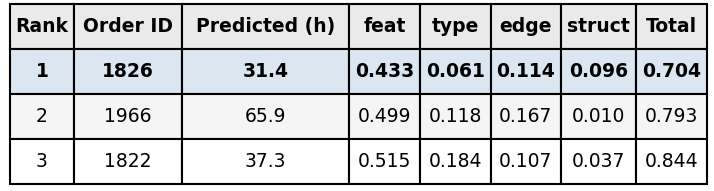
\includegraphics[width=1\textwidth]{figures/cf_showcase_candidates_table.png}
            \caption{Table showing the other possible counterfactual graph candidates found in the candidate set with their prediction value and dissimilarity scores}
            \label{fig:cf_candidates}
        \end{figure}
        
        In order to provide the stakeholder with a more actionable way of interpreting this explanation the different elements evaluated for the dissimilarity score are also shown in their own dedicated tables, highlighting the differences between them in the two subgraphs. For example, Fig. \ref{fig:cf_vwpnt_diff} and Fig. \ref{fig:cf_event_diff} show the difference in feature values between the Orders node and the Event nodes of the subgraphs respectively. Given that the dissimilarity was mainly driven by differences in features those different features are identified in this tables and shown to the stakeholder so they may better understand what's driving the model's predictions. 

        \begin{figure}[t!]
            \centering
            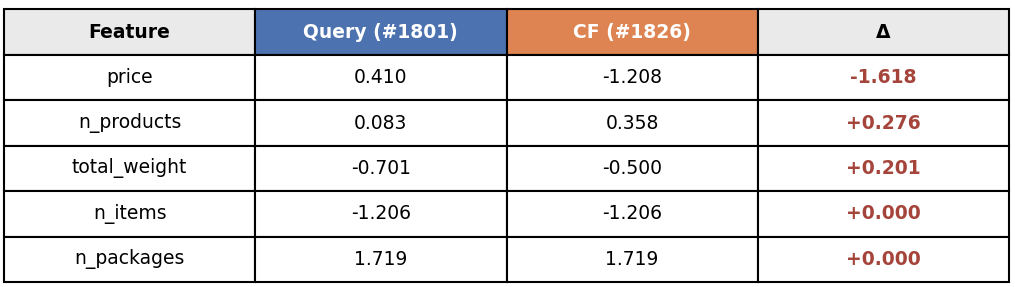
\includegraphics[width=1\textwidth]{figures/cf_showcase_viewpoint_feature_diff.png}
            \caption{Table showing the differences in the features of the Orders node of the two subgraphs. The total delta of the values is shown in the final column.}
            \label{fig:cf_vwpnt_diff}
        \end{figure}

        \begin{figure}[t!]
            \centering
            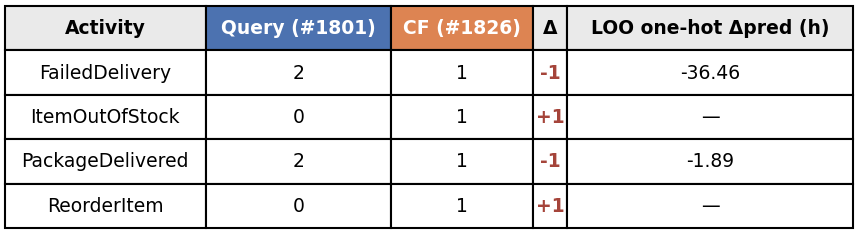
\includegraphics[width=1\textwidth]{figures/cf_showcase_event_type_diff.png}
            \caption{Table showing the differences in the features of the Event nodes of the two subgraphs. The number of events of each type is shown for the designated graph along with an estimation of their impact on the model's prediction.}
            \label{fig:cf_event_diff}
        \end{figure}

    \subsection{Explanation metrics}
        \begin{figure}[t!]
            \centering
            
\includegraphics[width=1\textwidth]{figures/explanation_quality_showcase_graphs.png}
            \caption{Graphs showing the baseline (full graph), fidelity+ (explanation removed), and fidelity- (explanation only) subgraphs used to compute the fidelity metrics meant for the stakeholder.}
            \label{fig:fidelity_graph}
        \end{figure}

        Finally, the stakeholder is also provided with fidelity metrics meant to help them assess the faithfulness of the explanation provided. An explanation is generated for the full graph using the framework and then the model's prediction is checked on a subgraph which does not contain the explanation subgraph (fidelity +) followed by a prediction performed on only the explanation subgraph (fidelity -). Fig. \ref{fig:fidelity_graph} shows the resulting baseline, fidelity+, and fidelity- graphs for one worked example, continuing the same order 1801 running example introduced earlier in this chapter. The stakeholder is shown only the resulting values for the given metrics, along with a short interpretation of the metric to aid them in their interpretation. Fig. \ref{fig:fidelity_table} shows the table of metrics. In this example the proposed explanation has a characterization score of 0.565 -- below the 0.815 aggregate LOO characterization reported for Order Management (Fig. \ref{fig:loo_comparison}) -- indicating that, while the proposed explanation is able to identify some of the input's most impactful elements, this particular trace is a comparatively less faithful case rather than the typical one. Its node sparsity value of 64.5\% and edge sparsity of 97.6\% indicate that the explanation has disregarded more than half of the existing nodes and almost all edges as unimportant to the model's prediction providing a very compact explanation subgraph.

        \begin{figure}[t!]
            \centering
            
\includegraphics[width=1\textwidth]{figures/explanation_quality_showcase_metrics_table.png}
            \caption{Table of the explanation metrics obtained.}
            \label{fig:fidelity_table}
        \end{figure}